\documentclass[11pt,fleqn]{article}
\usepackage{aip491}
\usepackage{graphicx} % Required for inserting images

\usepackage{booktabs}
\usepackage{amsfonts,amsmath,amssymb}
\usepackage{siunitx}
\usepackage{multirow}
\usepackage{cleveref}

\usepackage{titlesec}
\usepackage{appendix}

% TikZ for architecture diagrams
\usepackage{tikz}
\usetikzlibrary{shapes.geometric, arrows.meta, positioning, fit, backgrounds, calc}

\newcommand{\sectionbreak}{\clearpage}

\advisor{Huynh Van Thong}  % Advisor
\coadvisor{Not applicable for this Course}  % Co-advisor
\gpname{Geo-SLM}
\cpcode{AIP491-SP26}
\gmemf{noname} %student name 1
\gmemsc{noname} %student name 2
\gmemth{Le Quang That - SE183256} %student name 3
\gmemnS{3}  % Number of students in group, should be 3 or 4

\title{Geo-SLM: Hybrid Neuro-Symbolic Chart Analysis with Geometric Calibration and Small Language Models}  % Project title
\graduateDate{HCMC, April 2026}

\begin{document}

\maketitle

\pagenumbering{roman}
\setstretch{1.08} %\doublespacing  % 
\tableofcontents

\cleardoublepage
\addcontentsline{toc}{section}{\listfigurename}
\listoffigures
\cleardoublepage
\addcontentsline{toc}{section}{\listtablename}
\listoftables
\cleardoublepage
\pagenumbering{arabic}

\section{Introduction}

\subsection{Background}

Charts and graphs are among the most common methods for presenting quantitative information
in scientific publications, business reports, and data dashboards. A typical research paper
contains between two and ten chart images, each encoding numerical relationships that are
critical for understanding experimental results. Despite advances in machine learning and
natural language processing, the task of automatically extracting structured numerical data
from chart images remains a significant challenge.

Current approaches to automatic chart understanding fall into two categories. The first
category uses \textbf{end-to-end multimodal models} such as DePlot \cite{liu2023deplot} and
MatCha \cite{lee2023matcha}, which feed chart images directly into large vision-language
models that predict data tables or answer questions. While these approaches benefit from the
generalization capabilities of large models, they suffer from a fundamental limitation:
the model \emph{estimates} numerical values from pixel patterns rather than \emph{measuring}
them from geometric structures. This leads to hallucination errors where the model fabricates
plausible but incorrect data points.

The second category relies on \textbf{rule-based geometric analysis}, such as ReVision
\cite{savva2011revision}, which uses Hough transforms and template matching to extract
values from specific chart types. These methods are precise when applicable but lack
generalizability across chart types and fail on noisy or complex layouts.

Neither paradigm alone is sufficient. End-to-end models lack geometric precision, while
rule-based systems lack the perceptual flexibility of neural networks and the semantic
understanding of language models. This gap motivates a \textbf{hybrid neuro-symbolic
approach} that combines the strengths of both paradigms.

Furthermore, existing chart understanding systems are designed almost exclusively for
English-language charts. In the Vietnamese context, academic publications, government
reports, and business dashboards increasingly use charts with Vietnamese labels, axis
titles, and legends -- including diacritical marks (e.g., ``Doanh thu'',
``Tỷ lệ phần trăm'',
``Biểu đồ cột''). No published
system addresses Vietnamese chart understanding with structured data extraction and
Vietnamese-language question answering. This project targets this gap by designing the
pipeline as a \textbf{language-extensible} system: the core geometric and neural
components are language-agnostic, while OCR configuration, prompt templates, and SLM
fine-tuning data serve as localization layers that can be switched to Vietnamese without
modifying core logic.

\subsection{Objective}

This project aims to design and implement \textbf{Geo-SLM}, a hybrid AI system for
extracting structured numerical data from chart images. The system combines three
complementary paradigms:

\begin{enumerate}
    \item \textbf{Deep Learning for perception}: YOLOv8 \cite{jocher2023yolov8} for chart
          detection and ResNet-18 \cite{he2016resnet} for chart type classification.
    \item \textbf{Classical geometry for precision}: RANSAC-based axis calibration
          \cite{fischler1981ransac}, Ramer-Douglas-Peucker polyline simplification
          \cite{douglas1973rdp, ramer1972rdp}, and skeleton-based structural analysis
          \cite{lee1994skeleton} using OpenCV \cite{bradski2000opencv}.
    \item \textbf{Small Language Model (SLM) for reasoning}: A fine-tuned Qwen-2.5-1.5B
          \cite{yang2024qwen2} using QLoRA \cite{dettmers2024qlora} for OCR correction,
          value validation, and natural language description generation.
\end{enumerate}

The specific objectives are:
\begin{itemize}
    \item Achieve chart detection mAP@0.5 $> 85\%$ and classification accuracy $> 90\%$.
    \item Extract structured data (axis values, data series, labels) from 8 chart types
          with extraction confidence $> 90\%$.
    \item Build a large-scale training dataset ($> 200{,}000$ samples) from academic papers
          for SLM fine-tuning.
    \item Demonstrate that the hybrid geometric-plus-AI approach outperforms pure end-to-end
          methods in numerical accuracy while running locally on consumer hardware
          (NVIDIA RTX 3060, 6~GB VRAM).
    \item Enable \textbf{Vietnamese-language chart question answering}: the system must
          process charts containing Vietnamese text and support interactive Q\&A in
          Vietnamese, leveraging the extensible pipeline architecture.
\end{itemize}

\subsection{Problem Statement}

Given a document (PDF or image) containing one or more chart images, the system must:

\begin{itemize}
    \item \textbf{Input}: A PDF document or image file (PNG, JPG) containing charts.
    \item \textbf{Output}: For each detected chart, a structured JSON object containing:
          chart type, title, axis labels, data series (named lists of $(x, y)$ points),
          natural language description, and confidence scores with full traceability
          to source coordinates. The system must also support Vietnamese-language
          question answering over extracted chart data.
    \item \textbf{Chart types}: 8 categories -- line, bar, scatter, pie, histogram, box,
          heatmap, and area.
    \item \textbf{Performance targets}: Detection mAP@0.5 $> 85\%$; Classification accuracy
          $> 90\%$; End-to-end extraction confidence $> 80\%$.
    \item \textbf{Deployment constraint}: Must run on a single consumer GPU (RTX 3060,
          6~GB VRAM) without requiring cloud API access for core inference.
\end{itemize}

\subsection{Scope and Limitations}

\textbf{In scope:}
\begin{itemize}
    \item Charts from academic papers (arXiv cs.CV, cs.LG, cs.AI) and Vietnamese-language
          documents.
    \item 8 chart types: line, bar, scatter, pie, histogram, box, heatmap, area.
    \item PDF and raster image inputs (PNG, JPG, TIFF, BMP).
    \item Structured data extraction with JSON output.
    \item Local inference using fine-tuned SLM (1.5B parameters).
    \item Vietnamese-language OCR, chart Q\&A, and description generation.
\end{itemize}

\textbf{Out of scope:}
\begin{itemize}
    \item Business dashboards, presentation slides, and infographics.
    \item 3D charts, Sankey diagrams, and multi-panel composite figures.
    \item Real-time streaming or interactive chart manipulation.
    \item DOCX and HTML input formats (planned for future work).
\end{itemize}

\textbf{Known limitations:}
\begin{itemize}
    \item The core training data is sourced from English academic publications; Vietnamese
          chart data is generated through the localization pipeline (see \Cref{sec:viet_loc}).
    \item Axis calibration requires at least two readable numeric tick labels; charts
          without visible axis numbers produce no calibrated values.
    \item The SLM fine-tuning is ongoing at the time of writing; final SLM evaluation
          results (both English and Vietnamese) will be supplemented upon completion.
    \item Vietnamese OCR accuracy depends on diacritical mark recognition quality,
          which varies across OCR engines and font styles.
\end{itemize}


\section{Project Management Plan}

This project is developed as an individual capstone by a single student.

\subsection{Team Structure and Roles}

The project is completed by one member who handles all responsibilities: system
architecture design, data collection, model training, pipeline implementation,
testing, documentation, and thesis writing. Version control is managed through
Git with conventional commit messages, and progress is tracked via weekly reports
to the course coordinator.

\subsection{Communication Plan}

Weekly progress updates are submitted following the course schedule. The project
documentation (architecture documents, progress reports, and experiment logs) is
maintained in the repository under \texttt{docs/}. Collaboration with the thesis
advisor uses Overleaf for LaTeX document review.
\section{Literature Review}

This section reviews existing methods for automatic chart understanding, organized by
approach paradigm. We analyze the strengths and limitations of each category to motivate
the hybrid design of Geo-SLM.

\subsection{End-to-End Multimodal Approaches}

Recent advances in vision-language models have enabled end-to-end chart understanding
systems that process chart images directly without explicit geometric decomposition.

\textbf{DePlot} \cite{liu2023deplot} employs a two-stage approach: a Pix2Struct model
translates the chart image into a linearized data table, which is then processed by a
large language model (LLM) for question answering. DePlot achieves competitive results
on the ChartQA benchmark \cite{masry2022chartqa} with one-shot prompting. However,
because the Pix2Struct model estimates tabular values from visual patterns, it is prone
to hallucination -- producing plausible but numerically incorrect entries, especially
for charts with dense data points or overlapping series.

\textbf{MatCha} \cite{lee2023matcha} extends the Pix2Struct architecture with two
pretraining objectives: math reasoning and chart derendering. The derendering task trains
the model to generate the underlying data table from a chart image, improving numerical
grounding. MatCha achieves strong results on both ChartQA and PlotQA \cite{methani2020plotqa}
benchmarks. Despite these improvements, the model remains a large (282M+ parameters)
encoder-decoder that requires significant compute resources and does not provide
interpretable intermediate outputs.

\textbf{ChartReader} \cite{chen2022chartreader} proposes a unified framework that
detects chart components (bars, lines, legend entries) using Faster R-CNN, then applies
heuristic rules to reconstruct the data table. This approach provides more interpretable
outputs than DePlot or MatCha, but its component detection relies heavily on annotated
training data and struggles with unconventional chart layouts.

\subsection{Classical Geometric Approaches}

Before deep learning, chart understanding relied on classical image processing and
geometric analysis.

\textbf{ReVision} \cite{savva2011revision} classifies charts using visual features and
extracts data from bar charts using Hough line detection. While fully deterministic and
interpretable, ReVision supports only a single chart type (bar) and requires strict
assumptions about chart layout (aligned bars, visible grid lines). The method fails
on scatter plots, line charts, and charts with non-standard aesthetics.

Other traditional approaches use contour detection, template matching, and projection
profiles to identify chart elements. These methods offer high precision for well-formatted
charts but lack robustness against the visual diversity found in real-world academic
publications.

\subsection{Object Detection for Document Analysis}

The YOLO family \cite{redmon2016yolo, jocher2023yolov8} has been widely adopted for
object detection tasks in document analysis. YOLOv8 provides real-time detection with
competitive accuracy, making it suitable for chart region localization within full-page
document images. For chart detection specifically, the single-class detection strategy
(detecting ``chart'' as one class) with a separate classification stage has been shown
to outperform multi-class detection, since YOLO excels at localization while dedicated
classifiers (e.g., ResNet-18 \cite{he2016resnet}) provide higher type-classification
accuracy.

\subsection{OCR and Text Extraction}

Optical character recognition is fundamental to extracting textual information from charts,
including axis labels, titles, legend entries, and tick mark values. PaddleOCR
\cite{du2020paddleocr} and EasyOCR \cite{jaided2020easyocr} are two widely-used
open-source frameworks supporting multi-language text detection and recognition.
In the context of chart analysis, OCR faces unique challenges: text may be rotated
(Y-axis labels), overlapping (dense tick marks), or embedded as vector graphics
(invisible to pixel-based OCR). Post-processing heuristics -- such as spatial role
classification (assigning text to title, axis, legend, or value roles based on position)
and common-error correction (e.g., ``O'' to ``0'', ``l'' to ``1'') -- are essential
for reliable chart text extraction.

\subsection{Small Language Models and Parameter-Efficient Fine-Tuning}

Large language models have demonstrated strong reasoning capabilities for chart
understanding, but their deployment on consumer hardware is impractical. Small language
models (SLMs) with 1--3 billion parameters offer a practical alternative. Qwen-2.5
\cite{yang2024qwen2} provides instruction-tuned models starting at 0.5B parameters,
with the 1.5B variant balancing capability and efficiency.

Parameter-efficient fine-tuning methods allow adapting these models to domain-specific
tasks without full retraining. LoRA \cite{hu2022lora} introduces low-rank decomposition
of weight update matrices, training only 0.1--1\% of model parameters. QLoRA
\cite{dettmers2024qlora} extends LoRA with 4-bit quantization (NF4 format), reducing
memory requirements to as low as 4~GB VRAM for a 1.5B-parameter model. This enables
fine-tuning and inference on consumer GPUs such as the NVIDIA RTX 3060 (6~GB VRAM).

\subsection{Summary and Research Gap}

\Cref{tab:related_work} summarizes the comparison of existing approaches.

\begin{table}[htbp]
\centering
\caption{Comparison of existing chart understanding methods.}
\label{tab:related_work}
\begin{tabular}{@{}lp{2.5cm}rrlc@{}}
\toprule
\textbf{Method} & \textbf{Approach} & \textbf{Value Acc.} & \textbf{Types} & \textbf{Model Size} & \textbf{Explainable} \\
\midrule
DePlot \cite{liu2023deplot}     & Pix2Struct + LLM       & $\sim$85\% & 5+ & 282M+ & No \\
MatCha \cite{lee2023matcha}     & Chart pretraining      & $\sim$80\% & 5+ & 282M+ & No \\
ChartReader \cite{chen2022chartreader} & Detection + rules & $\sim$75\% & 3  & N/A   & Partial \\
ReVision \cite{savva2011revision}      & Hough transform   & $\sim$70\% & 1  & N/A   & Yes \\
\midrule
\textbf{Geo-SLM (Ours)} & \textbf{Hybrid neuro-symbolic} & \textbf{Target $>$95\%} & \textbf{8} & \textbf{1.5B} & \textbf{Yes} \\
\bottomrule
\end{tabular}
\end{table}

The key research gap is the absence of a system that combines:
\begin{enumerate}
    \item \textbf{Neural perception} for robust detection and classification across chart types,
    \item \textbf{Geometric measurement} for deterministic, traceable value extraction, and
    \item \textbf{Local SLM reasoning} for semantic understanding without cloud dependency.
\end{enumerate}

Geo-SLM addresses this gap by integrating all three paradigms in a modular, 5-stage
pipeline where each component operates on well-defined schema contracts, enabling
independent development, testing, and replacement of any component.


\section{Methodology}

This section describes the data collection pipeline and the overall approach used in
Geo-SLM. The data subsection covers the construction of the training dataset from raw
academic papers. The approach subsection presents the 5-stage hybrid pipeline architecture.

% ============================================================
\subsection{Data}
% ============================================================

\subsubsection{Data Collection Pipeline}

The training data is collected from approximately 4,000 academic papers in the cs.CV,
cs.LG, and cs.AI categories on arXiv. The collection pipeline transforms raw PDFs into
a structured SLM training dataset through six sequential stages, as illustrated in
\Cref{fig:data_pipeline}.

\begin{figure}[htbp]
\centering
% TikZ: Data Collection Pipeline Flow
% Usage: % TikZ: Data Collection Pipeline Flow
% Usage: \input{figures/tikz/tikz_data_pipeline.tex}
% Requires: \usepackage{tikz} \usetikzlibrary{shapes.geometric, arrows.meta, positioning, fit, backgrounds}

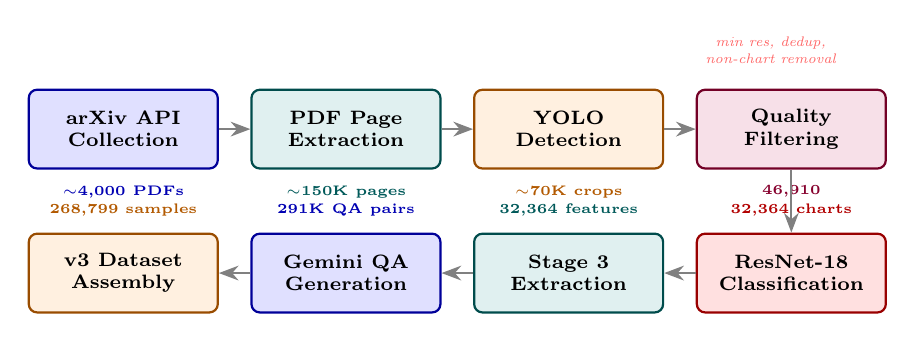
\begin{tikzpicture}[
    node distance=0.5cm and 0.4cm,
    step/.style={
        rectangle, rounded corners=3pt, draw=#1!60!black, thick,
        minimum width=2.4cm, minimum height=1.0cm,
        fill=#1!12, font=\scriptsize\bfseries, align=center
    },
    count/.style={
        font=\tiny\bfseries, text=#1!70!black, align=center
    },
    arrow/.style={-{Stealth[length=2.5mm]}, thick, draw=black!50},
    filter/.style={font=\tiny\itshape, text=red!60, align=center}
]

% Row 1
\node[step=blue] (arxiv) {arXiv API\\Collection};
\node[step=teal, right=of arxiv] (pdf) {PDF Page\\Extraction};
\node[step=orange, right=of pdf] (yolo) {YOLO\\Detection};

% Row 2
\node[step=purple, right=of yolo] (filter) {Quality\\Filtering};
\node[step=red, below=0.8cm of filter] (classify) {ResNet-18\\Classification};
\node[step=teal, left=of classify] (s3) {Stage 3\\Extraction};

% Row 3
\node[step=blue, left=of s3] (qa) {Gemini QA\\Generation};
\node[step=orange, left=of qa] (dataset) {v3 Dataset\\Assembly};

% Counts
\node[count=blue, below=0.08cm of arxiv] {$\sim$4,000 PDFs};
\node[count=teal, below=0.08cm of pdf] {$\sim$150K pages};
\node[count=orange, below=0.08cm of yolo] {$\sim$70K crops};
\node[count=purple, below=0.08cm of filter] {46,910};
\node[count=red, above=0.08cm of classify] {32,364 charts};
\node[count=teal, above=0.08cm of s3] {32,364 features};
\node[count=blue, above=0.08cm of qa] {291K QA pairs};
\node[count=orange, above=0.08cm of dataset] {268,799 samples};

% Arrows
\draw[arrow] (arxiv) -- (pdf);
\draw[arrow] (pdf) -- (yolo);
\draw[arrow] (yolo) -- (filter);
\draw[arrow] (filter) -- (classify);
\draw[arrow] (classify) -- (s3);
\draw[arrow] (s3) -- (qa);
\draw[arrow] (qa) -- (dataset);

% Filter annotations
\node[filter, above=0.2cm of filter.north west, anchor=south west] {min res, dedup,\\non-chart removal};

\end{tikzpicture}

% Requires: \usepackage{tikz} \usetikzlibrary{shapes.geometric, arrows.meta, positioning, fit, backgrounds}

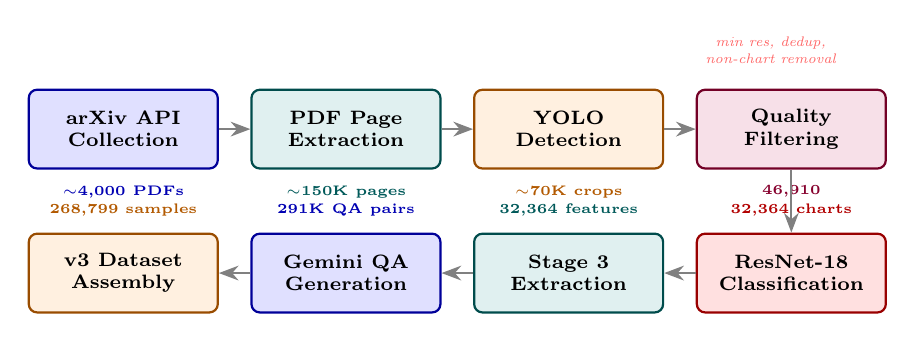
\begin{tikzpicture}[
    node distance=0.5cm and 0.4cm,
    step/.style={
        rectangle, rounded corners=3pt, draw=#1!60!black, thick,
        minimum width=2.4cm, minimum height=1.0cm,
        fill=#1!12, font=\scriptsize\bfseries, align=center
    },
    count/.style={
        font=\tiny\bfseries, text=#1!70!black, align=center
    },
    arrow/.style={-{Stealth[length=2.5mm]}, thick, draw=black!50},
    filter/.style={font=\tiny\itshape, text=red!60, align=center}
]

% Row 1
\node[step=blue] (arxiv) {arXiv API\\Collection};
\node[step=teal, right=of arxiv] (pdf) {PDF Page\\Extraction};
\node[step=orange, right=of pdf] (yolo) {YOLO\\Detection};

% Row 2
\node[step=purple, right=of yolo] (filter) {Quality\\Filtering};
\node[step=red, below=0.8cm of filter] (classify) {ResNet-18\\Classification};
\node[step=teal, left=of classify] (s3) {Stage 3\\Extraction};

% Row 3
\node[step=blue, left=of s3] (qa) {Gemini QA\\Generation};
\node[step=orange, left=of qa] (dataset) {v3 Dataset\\Assembly};

% Counts
\node[count=blue, below=0.08cm of arxiv] {$\sim$4,000 PDFs};
\node[count=teal, below=0.08cm of pdf] {$\sim$150K pages};
\node[count=orange, below=0.08cm of yolo] {$\sim$70K crops};
\node[count=purple, below=0.08cm of filter] {46,910};
\node[count=red, above=0.08cm of classify] {32,364 charts};
\node[count=teal, above=0.08cm of s3] {32,364 features};
\node[count=blue, above=0.08cm of qa] {291K QA pairs};
\node[count=orange, above=0.08cm of dataset] {268,799 samples};

% Arrows
\draw[arrow] (arxiv) -- (pdf);
\draw[arrow] (pdf) -- (yolo);
\draw[arrow] (yolo) -- (filter);
\draw[arrow] (filter) -- (classify);
\draw[arrow] (classify) -- (s3);
\draw[arrow] (s3) -- (qa);
\draw[arrow] (qa) -- (dataset);

% Filter annotations
\node[filter, above=0.2cm of filter.north west, anchor=south west] {min res, dedup,\\non-chart removal};

\end{tikzpicture}

\caption{Data collection pipeline: from arXiv papers to SLM training dataset.
    Each stage filters and transforms the data, reducing volume while increasing quality.}
\label{fig:data_pipeline}
\end{figure}

\Cref{tab:data_scale} summarizes the scale at each stage of the pipeline.

\begin{table}[htbp]
\centering
\caption{Data pipeline scale at each processing stage.}
\label{tab:data_scale}
\begin{table}[htbp]
\centering
\caption{Data Collection Pipeline Scale}
\label{tab:data-pipeline-scale}
\begin{tabular}{@{}lr@{}}
\toprule
\textbf{Stage} & \textbf{Count} \\
\midrule
arXiv PDFs processed      &  $\sim$4,000 \\
Raw page images           & $\sim$150,000 \\
Candidate chart regions   &  $\sim$70,000 \\
After quality filtering   &     46,910 \\
Final classified charts   &     32,364 \\
OCR cache entries         &     46,910 \\
SLM training samples (v3) &    268,799 \\
\bottomrule
\end{tabular}
\end{table}
\end{table}

\textbf{Step 1: PDF Mining.}
PyMuPDF renders each PDF page at 150~DPI, producing approximately 150,000 page images.
The ArXiv API is accessed with rate limiting ($\sim$3s between requests) and resume
capability via progress files.

\textbf{Step 2: Chart Detection.}
A trained YOLOv8m model (confidence threshold 0.5) detects chart regions in each page
image, yielding approximately 70,000 candidate chart crops.

\textbf{Step 3: Classification and Filtering.}
A cascade classifier (ResNet-18 primary, rule-based fallback) assigns each crop to one
of 8 chart types: line, bar, scatter, pie, histogram, box, heatmap, and area. After
filtering low-confidence detections and duplicates, 32,364 verified charts remain.
\Cref{tab:chart_dist} shows the distribution by type.

\begin{table}[htbp]
\centering
\caption{Chart type distribution in the classified dataset (32,364 charts).}
\label{tab:chart_dist}
\begin{tabular}{@{}lrr@{}}
\toprule
\textbf{Chart Type} & \textbf{Count} & \textbf{Share (\%)} \\
\midrule
line      & 10,036 & 31.0 \\
bar       &  9,086 & 28.1 \\
box       &  4,867 & 15.0 \\
scatter   &  2,802 &  8.7 \\
pie       &  2,421 &  7.5 \\
histogram &  2,060 &  6.4 \\
heatmap   &    680 &  2.1 \\
area      &    412 &  1.3 \\
\midrule
\textbf{Total} & \textbf{32,364} & \textbf{100.0} \\
\bottomrule
\end{tabular}
\end{table}

\textbf{Step 4: Feature Extraction.}
The Stage~3 extraction pipeline (see \Cref{sec:system_s3}) processes all 32,364 charts
using parallel batch execution. The extraction achieves 100\% success rate with 0\%
data corruption, producing structured feature JSONs containing axis calibration,
OCR text with spatial roles, detected elements, and confidence scores.

\textbf{Step 5: QA Generation.}
The \texttt{data\_factory} tool uses Gemini 2.0 Flash API to generate 10 questions per
chart across four difficulty levels: shallow (25\%), intermediate (35\%), deep (30\%),
and conceptual (10\%). This produces approximately 291,000 QA pairs. Cross-validation
confirms 87\% text overlap between Stage~3 features and QA answers.

\textbf{Step 6: Dataset Assembly.}
The final SLM training dataset (v3) is assembled by merging Stage~3 features with QA
pairs, formatted as ChatML conversations. The dataset is split by \texttt{chart\_id}
to prevent data leakage between train, validation, and test sets.

\subsubsection{SLM Training Dataset}

\Cref{tab:splits} shows the dataset split statistics.

\begin{table}[htbp]
\centering
\caption{SLM training dataset v3 split statistics.}
\label{tab:splits}
\begin{tabular}{@{}lrr@{}}
\toprule
\textbf{Split} & \textbf{Samples} & \textbf{Ratio (\%)} \\
\midrule
Train      & 228,494 & 85 \\
Validation &  26,888 & 10 \\
Test       &  13,417 &  5 \\
\midrule
\textbf{Total} & \textbf{268,799} & \textbf{100} \\
\bottomrule
\end{tabular}
\end{table}

The v3 dataset represents a 9.9$\times$ improvement over v2 (27,159 $\to$ 268,799
samples), achieved by fixing axis key format errors (coverage increased from 4\%
to 69.9\%), ensuring 100\% Stage~3 feature coverage, and implementing chart-ID-based
splitting to eliminate data leakage.

\Cref{fig:data_funnel} visualizes the data reduction funnel across pipeline stages.

\begin{figure}[htbp]
\centering
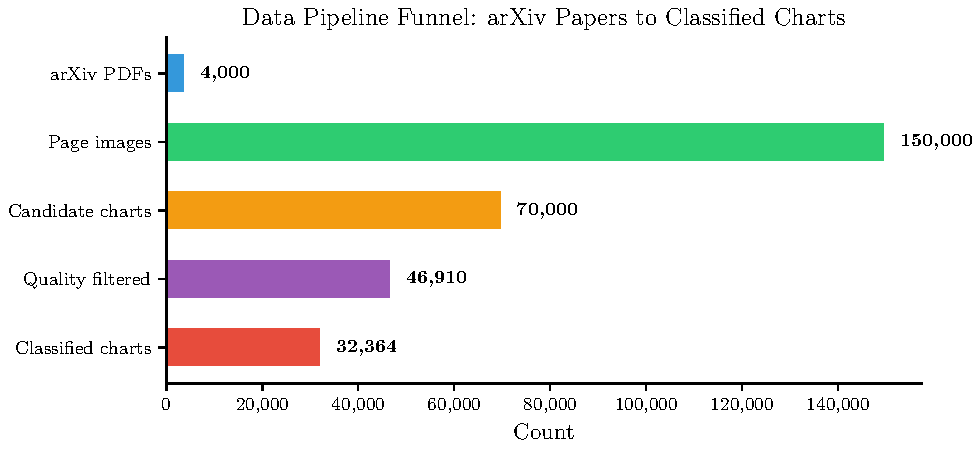
\includegraphics[width=0.85\textwidth]{figures/fig_data_pipeline_funnel.pdf}
\caption{Data pipeline funnel: volume at each stage from raw PDFs to final dataset.}
\label{fig:data_funnel}
\end{figure}

\subsubsection{SLM Fine-Tuning Configuration}

The SLM is fine-tuned using QLoRA \cite{dettmers2024qlora} on the Qwen-2.5-1.5B-Instruct
base model \cite{yang2024qwen2}. \Cref{tab:slm_config} lists the training hyperparameters.

\begin{table}[htbp]
\centering
\caption{SLM fine-tuning configuration (QLoRA).}
\label{tab:slm_config}
\begin{tabular}{@{}ll@{}}
\toprule
\textbf{Parameter} & \textbf{Value} \\
\midrule
Base model       & Llama-3.2-1B-Instruct \\
Method           & QLoRA (4-bit NF4 + LoRA rank 16) \\
LoRA targets     & q, k, v, o, gate, up, down projections \\
Optimizer        & paged\_adamw\_32bit \\
LR scheduler     & Cosine (warmup 5\%) \\
VRAM requirement & $\sim$4--5 GB (RTX 3060 6GB) \\
Batch size       & 2 (effective 16 with gradient accumulation 8) \\
Learning rate    & $2 \times 10^{-4}$ \\
Max seq.\ length & 1024 tokens \\
Precision        & bf16 (mixed precision) \\
Weight decay     & 0.01 \\
LoRA dropout     & 0.05 \\
\bottomrule
\end{tabular}
\end{table}

The QLoRA configuration uses 4-bit NF4 quantization with LoRA rank~16, resulting in
11.27M trainable parameters (0.9\% of total). This fits within the 6~GB VRAM constraint
of an NVIDIA RTX~3060. Training follows a 4-stage curriculum: (1) chart type and axis
labels, (2) value extraction and OCR correction, (3) trends and comparisons, and
(4) noisy OCR and complex layouts.

% ============================================================
\subsection{Approach}
% ============================================================

\subsubsection{Hybrid Neuro-Symbolic Design}

The core hypothesis of Geo-SLM is that treating charts as \textbf{geometric entities}
rather than pixel patterns yields higher extraction accuracy than pure end-to-end
multimodal approaches. The system combines three complementary paradigms:

\begin{itemize}
    \item \textbf{Deep Learning} for perception: detecting chart regions (YOLOv8) and
          classifying chart types (ResNet-18).
    \item \textbf{Symbolic/Geometric Analysis} for precision: calibrating axes (RANSAC),
          simplifying curves (RDP), and mapping pixel coordinates to data values.
    \item \textbf{Language Model Reasoning} for understanding: correcting OCR errors,
          validating extracted data, and generating natural language descriptions.
\end{itemize}

\Cref{fig:approach_cmp} contrasts the traditional end-to-end approach with the Geo-SLM
hybrid approach.

\begin{figure}[htbp]
\centering
% TikZ: Hybrid Approach Comparison (Traditional vs Geo-SLM)
% Usage: % TikZ: Hybrid Approach Comparison (Traditional vs Geo-SLM)
% Usage: \input{figures/tikz/tikz_approach_comparison.tex}
% Requires: \usepackage{tikz} \usetikzlibrary{shapes.geometric, arrows.meta, positioning, fit, backgrounds, calc}

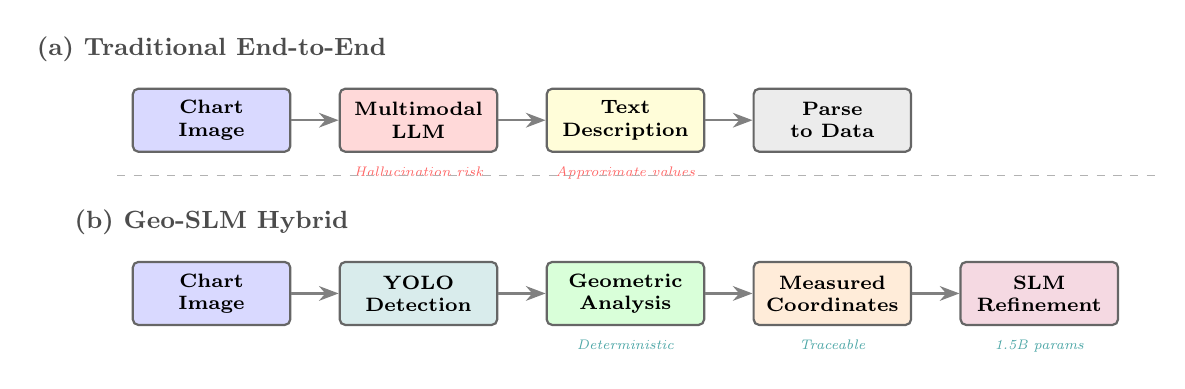
\begin{tikzpicture}[
    node distance=0.4cm and 0.6cm,
    block/.style={
        rectangle, rounded corners=2pt, draw=black!60, thick,
        minimum width=2.0cm, minimum height=0.8cm,
        font=\scriptsize\bfseries, align=center
    },
    arrow/.style={-{Stealth[length=2.5mm]}, thick, draw=black!50},
    grouplabel/.style={font=\small\bfseries, text=black!70},
    prob/.style={font=\tiny\itshape, text=red!60},
    good/.style={font=\tiny\itshape, text=teal!70}
]

% Traditional approach (top)
\node[grouplabel] (trad_label) at (0, 2.5) {(a) Traditional End-to-End};

\node[block, fill=blue!15] (t_img) at (0, 1.6) {Chart\\Image};
\node[block, fill=red!15, right=of t_img] (t_llm) {Multimodal\\LLM};
\node[block, fill=yellow!15, right=of t_llm] (t_text) {Text\\Description};
\node[block, fill=gray!15, right=of t_text] (t_parse) {Parse\\to Data};

\draw[arrow] (t_img) -- (t_llm);
\draw[arrow] (t_llm) -- (t_text);
\draw[arrow] (t_text) -- (t_parse);

\node[prob, below=0.05cm of t_llm] {Hallucination risk};
\node[prob, below=0.05cm of t_text] {Approximate values};

% Geo-SLM approach (bottom)
\node[grouplabel] at (0, 0.3) {(b) Geo-SLM Hybrid};

\node[block, fill=blue!15] (g_img) at (0, -0.6) {Chart\\Image};
\node[block, fill=teal!15, right=of g_img] (g_yolo) {YOLO\\Detection};
\node[block, fill=green!15, right=of g_yolo] (g_geo) {Geometric\\Analysis};
\node[block, fill=orange!15, right=of g_geo] (g_coord) {Measured\\Coordinates};
\node[block, fill=purple!15, right=of g_coord] (g_slm) {SLM\\Refinement};

\draw[arrow] (g_img) -- (g_yolo);
\draw[arrow] (g_yolo) -- (g_geo);
\draw[arrow] (g_geo) -- (g_coord);
\draw[arrow] (g_coord) -- (g_slm);

\node[good, below=0.05cm of g_geo] {Deterministic};
\node[good, below=0.05cm of g_coord] {Traceable};
\node[good, below=0.05cm of g_slm] {1.5B params};

% Divider
\draw[dashed, black!30] (-1.2, 0.9) -- (12, 0.9);

\end{tikzpicture}

% Requires: \usepackage{tikz} \usetikzlibrary{shapes.geometric, arrows.meta, positioning, fit, backgrounds, calc}

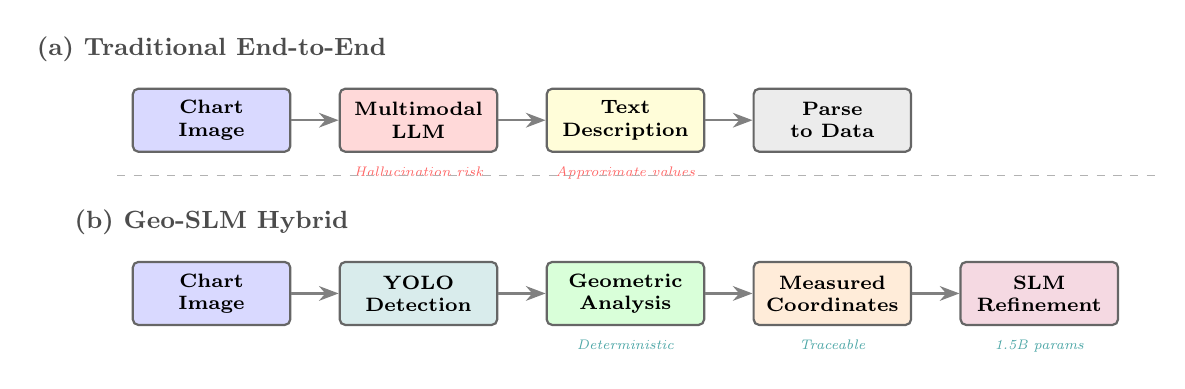
\begin{tikzpicture}[
    node distance=0.4cm and 0.6cm,
    block/.style={
        rectangle, rounded corners=2pt, draw=black!60, thick,
        minimum width=2.0cm, minimum height=0.8cm,
        font=\scriptsize\bfseries, align=center
    },
    arrow/.style={-{Stealth[length=2.5mm]}, thick, draw=black!50},
    grouplabel/.style={font=\small\bfseries, text=black!70},
    prob/.style={font=\tiny\itshape, text=red!60},
    good/.style={font=\tiny\itshape, text=teal!70}
]

% Traditional approach (top)
\node[grouplabel] (trad_label) at (0, 2.5) {(a) Traditional End-to-End};

\node[block, fill=blue!15] (t_img) at (0, 1.6) {Chart\\Image};
\node[block, fill=red!15, right=of t_img] (t_llm) {Multimodal\\LLM};
\node[block, fill=yellow!15, right=of t_llm] (t_text) {Text\\Description};
\node[block, fill=gray!15, right=of t_text] (t_parse) {Parse\\to Data};

\draw[arrow] (t_img) -- (t_llm);
\draw[arrow] (t_llm) -- (t_text);
\draw[arrow] (t_text) -- (t_parse);

\node[prob, below=0.05cm of t_llm] {Hallucination risk};
\node[prob, below=0.05cm of t_text] {Approximate values};

% Geo-SLM approach (bottom)
\node[grouplabel] at (0, 0.3) {(b) Geo-SLM Hybrid};

\node[block, fill=blue!15] (g_img) at (0, -0.6) {Chart\\Image};
\node[block, fill=teal!15, right=of g_img] (g_yolo) {YOLO\\Detection};
\node[block, fill=green!15, right=of g_yolo] (g_geo) {Geometric\\Analysis};
\node[block, fill=orange!15, right=of g_geo] (g_coord) {Measured\\Coordinates};
\node[block, fill=purple!15, right=of g_coord] (g_slm) {SLM\\Refinement};

\draw[arrow] (g_img) -- (g_yolo);
\draw[arrow] (g_yolo) -- (g_geo);
\draw[arrow] (g_geo) -- (g_coord);
\draw[arrow] (g_coord) -- (g_slm);

\node[good, below=0.05cm of g_geo] {Deterministic};
\node[good, below=0.05cm of g_coord] {Traceable};
\node[good, below=0.05cm of g_slm] {1.5B params};

% Divider
\draw[dashed, black!30] (-1.2, 0.9) -- (12, 0.9);

\end{tikzpicture}

\caption{Comparison of traditional end-to-end approach (top) vs.\ Geo-SLM hybrid
    neuro-symbolic approach (bottom). Geo-SLM uses geometric measurement for precision
    and SLM reasoning for semantic understanding.}
\label{fig:approach_cmp}
\end{figure}

\subsubsection{5-Stage Pipeline Architecture}

The system is organized as a modular 5-stage pipeline where each stage has well-defined
input and output schema contracts (Pydantic v2 frozen models). \Cref{fig:pipeline_arch}
shows the pipeline architecture.

\begin{figure}[htbp]
\centering
% TikZ: 5-Stage Pipeline Architecture
% Usage: % TikZ: 5-Stage Pipeline Architecture
% Usage: \input{figures/tikz/tikz_pipeline_architecture.tex}
% Requires: \usepackage{tikz} \usetikzlibrary{shapes.geometric, arrows.meta, positioning, fit, backgrounds}

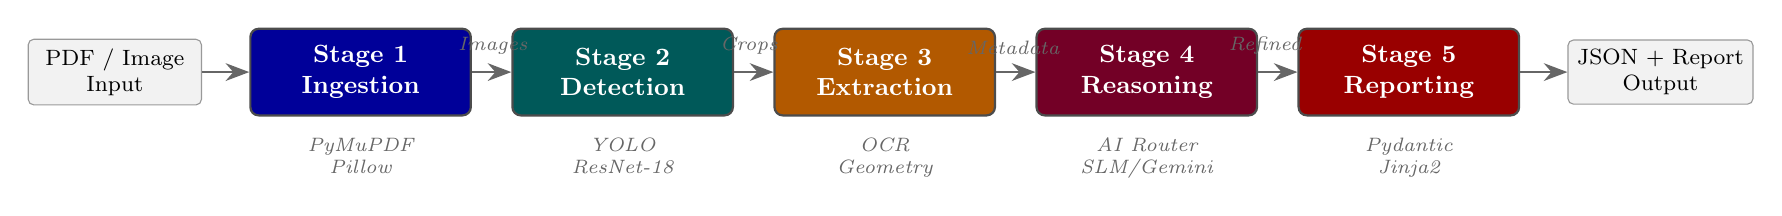
\begin{tikzpicture}[
    node distance=0.8cm and 0.5cm,
    stage/.style={
        rectangle, rounded corners=3pt, draw=black!70, thick,
        minimum width=2.8cm, minimum height=1.1cm,
        font=\small\bfseries, text=white, align=center
    },
    io/.style={
        rectangle, rounded corners=2pt, draw=black!40,
        minimum width=2.2cm, minimum height=0.7cm,
        font=\footnotesize, fill=black!5, align=center
    },
    arrow/.style={-{Stealth[length=3mm]}, thick, draw=black!60},
    label/.style={font=\scriptsize\itshape, text=black!60, align=center}
]

% Stages
\node[stage, fill=blue!60!black] (s1) {Stage 1\\Ingestion};
\node[stage, fill=teal!70!black, right=of s1] (s2) {Stage 2\\Detection};
\node[stage, fill=orange!70!black, right=of s2] (s3) {Stage 3\\Extraction};
\node[stage, fill=purple!60!black, right=of s3] (s4) {Stage 4\\Reasoning};
\node[stage, fill=red!60!black, right=of s4] (s5) {Stage 5\\Reporting};

% Arrows between stages
\draw[arrow] (s1) -- (s2);
\draw[arrow] (s2) -- (s3);
\draw[arrow] (s3) -- (s4);
\draw[arrow] (s4) -- (s5);

% Input/Output
\node[io, left=0.6cm of s1] (input) {PDF / Image\\Input};
\node[io, right=0.6cm of s5] (output) {JSON + Report\\Output};
\draw[arrow] (input) -- (s1);
\draw[arrow] (s5) -- (output);

% Labels below stages
\node[label, below=0.15cm of s1] {PyMuPDF\\Pillow};
\node[label, below=0.15cm of s2] {YOLO\\ResNet-18};
\node[label, below=0.15cm of s3] {OCR\\Geometry};
\node[label, below=0.15cm of s4] {AI Router\\SLM/Gemini};
\node[label, below=0.15cm of s5] {Pydantic\\Jinja2};

% Data labels above arrows
\node[label, above=0.1cm of s1.east, anchor=south west, xshift=-0.3cm] {Images};
\node[label, above=0.1cm of s2.east, anchor=south west, xshift=-0.3cm] {Crops};
\node[label, above=0.1cm of s3.east, anchor=south west, xshift=-0.5cm] {Metadata};
\node[label, above=0.1cm of s4.east, anchor=south west, xshift=-0.5cm] {Refined};

\end{tikzpicture}

% Requires: \usepackage{tikz} \usetikzlibrary{shapes.geometric, arrows.meta, positioning, fit, backgrounds}

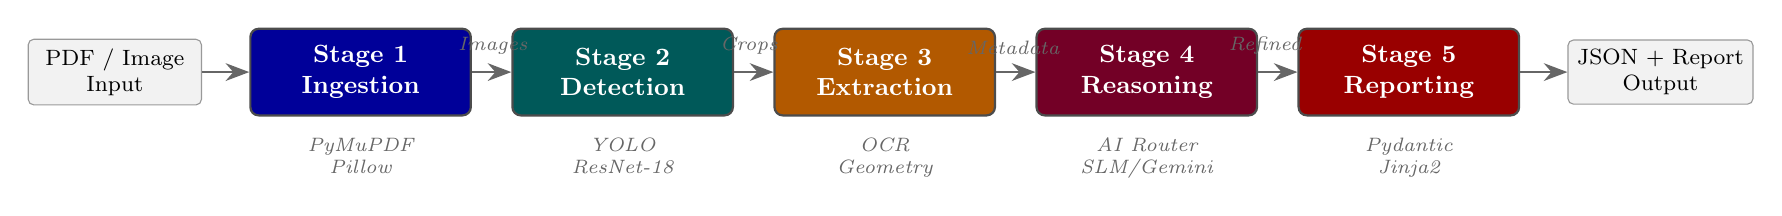
\begin{tikzpicture}[
    node distance=0.8cm and 0.5cm,
    stage/.style={
        rectangle, rounded corners=3pt, draw=black!70, thick,
        minimum width=2.8cm, minimum height=1.1cm,
        font=\small\bfseries, text=white, align=center
    },
    io/.style={
        rectangle, rounded corners=2pt, draw=black!40,
        minimum width=2.2cm, minimum height=0.7cm,
        font=\footnotesize, fill=black!5, align=center
    },
    arrow/.style={-{Stealth[length=3mm]}, thick, draw=black!60},
    label/.style={font=\scriptsize\itshape, text=black!60, align=center}
]

% Stages
\node[stage, fill=blue!60!black] (s1) {Stage 1\\Ingestion};
\node[stage, fill=teal!70!black, right=of s1] (s2) {Stage 2\\Detection};
\node[stage, fill=orange!70!black, right=of s2] (s3) {Stage 3\\Extraction};
\node[stage, fill=purple!60!black, right=of s3] (s4) {Stage 4\\Reasoning};
\node[stage, fill=red!60!black, right=of s4] (s5) {Stage 5\\Reporting};

% Arrows between stages
\draw[arrow] (s1) -- (s2);
\draw[arrow] (s2) -- (s3);
\draw[arrow] (s3) -- (s4);
\draw[arrow] (s4) -- (s5);

% Input/Output
\node[io, left=0.6cm of s1] (input) {PDF / Image\\Input};
\node[io, right=0.6cm of s5] (output) {JSON + Report\\Output};
\draw[arrow] (input) -- (s1);
\draw[arrow] (s5) -- (output);

% Labels below stages
\node[label, below=0.15cm of s1] {PyMuPDF\\Pillow};
\node[label, below=0.15cm of s2] {YOLO\\ResNet-18};
\node[label, below=0.15cm of s3] {OCR\\Geometry};
\node[label, below=0.15cm of s4] {AI Router\\SLM/Gemini};
\node[label, below=0.15cm of s5] {Pydantic\\Jinja2};

% Data labels above arrows
\node[label, above=0.1cm of s1.east, anchor=south west, xshift=-0.3cm] {Images};
\node[label, above=0.1cm of s2.east, anchor=south west, xshift=-0.3cm] {Crops};
\node[label, above=0.1cm of s3.east, anchor=south west, xshift=-0.5cm] {Metadata};
\node[label, above=0.1cm of s4.east, anchor=south west, xshift=-0.5cm] {Refined};

\end{tikzpicture}

\caption{Geo-SLM 5-stage pipeline architecture with input/output types and
    representative technologies at each stage.}
\label{fig:pipeline_arch}
\end{figure}

\Cref{tab:stages} summarizes the responsibilities of each stage.

\begin{table}[htbp]
\centering
\caption{Pipeline stages: input, output, and key technologies.}
\label{tab:stages}
\begin{table}[htbp]
\centering
\caption{Pipeline Stage Summary}
\label{tab:pipeline-stages}
\begin{tabular}{@{}clp{3cm}p{3cm}l@{}}
\toprule
\textbf{Stage} & \textbf{Name} & \textbf{Input} & \textbf{Output} & \textbf{Key Library} \\
\midrule
1 & Ingestion   & PDF, DOCX, PNG, JPG     & Clean page images        & PyMuPDF, Pillow \\
2 & Detection   & Page images             & Cropped charts + BBoxes  & Ultralytics YOLO \\
3 & Extraction  & Cropped chart           & Raw metadata (OCR, geometry) & EasyOCR, OpenCV \\
4 & Reasoning   & Metadata + chart image  & Refined structured data  & AI Router (SLM/Gemini) \\
5 & Reporting   & Refined data            & JSON + Markdown report   & Pydantic, Jinja2 \\
\bottomrule
\end{tabular}
\end{table}
\end{table}

Each stage inherits from \texttt{BaseStage[InputT,~OutputT]}, a generic abstract base
class that enforces input validation, provides fallback behavior for graceful degradation,
and enables independent testing. The pipeline orchestrator executes stages sequentially,
passing validated output from one stage as input to the next.

\subsubsection{AI Routing with Fallback Chains}

Stage~4 reasoning uses an \textbf{AI Router} that decouples task-level logic from
provider selection. Each task type (OCR correction, value mapping, chart reasoning,
description generation) has a configurable fallback chain. The default chain prioritizes
local SLM inference (zero cost, no network dependency) with automatic fallback to
cloud APIs (Gemini, OpenAI) when local confidence is below threshold.

This routing architecture is implemented using the \textbf{Adapter Pattern}: all AI
providers implement a common \texttt{BaseAIAdapter} interface, and the Router walks
the fallback chain until a provider succeeds or all options are exhausted.

\subsubsection{Configuration-Driven Design}

All model paths, detection thresholds, stage toggles, and AI routing chains are
externalized to YAML configuration files (OmegaConf). This enables experiment
reproducibility and parameter tuning without code modifications. The configuration
hierarchy consists of four files: \texttt{base.yaml} (shared settings),
\texttt{models.yaml} (model paths and AI routing), \texttt{pipeline.yaml}
(stage parameters), and \texttt{training.yaml} (SLM fine-tuning).

% ============================================================
\subsection{Vietnamese Language Integration Strategy}
\label{sec:viet_loc}
% ============================================================

A primary objective of this project is to enable chart question answering in Vietnamese.
Rather than building a Vietnamese-specific system from scratch, the architecture follows
a \textbf{Core-first, Localize-second} strategy: the entire pipeline is developed and
validated with English data first, then extended to Vietnamese through configuration
changes and data generation -- without modifying core pipeline logic. This approach
adheres to the Open/Closed Principle and reduces the risk of conflating pipeline bugs
with language-specific issues.

\subsubsection{Localization Architecture}

Vietnamese support requires changes at three layers of the pipeline, while the geometric
core (skeleton extraction, RDP vectorization, RANSAC calibration, element detection)
remains entirely language-agnostic:

\begin{table}[htbp]
\centering
\caption{Vietnamese localization touchpoints across the pipeline.}
\label{tab:viet_touchpoints}
\begin{tabular}{@{}clll@{}}
\toprule
\textbf{Stage} & \textbf{Component} & \textbf{Change Required} & \textbf{Core Modified?} \\
\midrule
S3 & OCR Engine config & Set language to \texttt{"vi"} or \texttt{["en","vi"]} & No (config only) \\
S3 & OCR role keywords & Add Vietnamese keywords (e.g., ``trục tung'') & Additive only \\
S3 & Geometric Mapper & No change (operates on pixel coordinates) & No \\
S3 & Classifier & No change (visual features, language-agnostic) & No \\
S4 & Prompt templates & Create Vietnamese prompt variants (\texttt{*\_vi.txt}) & No (new files) \\
S4 & \texttt{output\_language} & Wire existing config field into prompt builder & Minimal \\
S4 & AI Router/Adapters & No change (language-transparent interface) & No \\
S5 & Report templates & Add Vietnamese summary templates & Additive only \\
Data & QA Generator prompts & Vietnamese QA generation instructions & Config only \\
Data & SLM training data & Generate 5,000--10,000 Vietnamese QA samples & New data \\
\bottomrule
\end{tabular}
\end{table}

\subsubsection{OCR for Vietnamese Diacritical Marks}

Vietnamese uses Latin script with an extensive diacritical system (6~tone marks $\times$
12~vowel variants), making accurate OCR critical. The current OCR engine
(\texttt{ocr\_engine.py}) supports language switching through configuration:

\begin{itemize}
    \item \textbf{PaddleOCR}: Natively supports Vietnamese (\texttt{lang="vi"}) with
          dedicated recognition weights trained on Vietnamese text corpora.
    \item \textbf{EasyOCR}: Supports Vietnamese (\texttt{languages=["vi"]}) with
          multi-language simultaneous recognition.
    \item \textbf{Tesseract}: Supports Vietnamese via \texttt{lang="vie"} tessdata files.
\end{itemize}

The configuration change is a single YAML update in \texttt{config/models.yaml}:
\texttt{ocr.paddleocr.lang: "vi"} (or \texttt{["en", "vi"]} for bilingual charts).
No Python code changes are required in the OCR engine itself.

However, Vietnamese diacritical marks introduce specific OCR challenges: confusion
between visually similar characters (e.g., ``O'' vs.\ ``\^{O}'',
``a'' vs.\ ``ă''), incorrect tone mark placement,
and merging of diacritics with nearby chart elements. These errors are addressed through
the SLM reasoning stage (Stage~4), where Vietnamese-specific OCR correction patterns
supplement the existing English correction table.

\subsubsection{Vietnamese Keyword Mapping for Role Classification}

The OCR role classifier in Stage~3 assigns spatial roles (title, axis label, legend,
value) to extracted text using a combination of positional heuristics and keyword matching.
The English keyword lists (e.g., ``count'', ``percentage'', ``legend'') must be extended
with Vietnamese equivalents:

\begin{itemize}
    \item \textbf{Axis labels}: ``số lượng'',
          ``tỷ lệ'',
          ``giá trị'',
          ``doanh thu'',
          ``thời gian'',
          ``năm''
    \item \textbf{Legend}: ``chú giải'',
          ``nhóm'',
          ``loại''
    \item \textbf{Title}: ``biểu đồ'',
          ``hình''
\end{itemize}

This is implemented as an additive extension to the existing keyword dictionaries,
preserving English support while enabling bilingual role detection.

\subsubsection{Vietnamese Prompt Templates and QA Generation}

For Stage~4 reasoning, the prompt template system supports language-specific variants:
\begin{itemize}
    \item System prompts are parameterized with an \texttt{output\_language} field
          (already defined in \texttt{PromptConfig} but currently unused for English-only
          operation).
    \item Vietnamese prompt files (\texttt{reasoning\_vi.txt}, \texttt{description\_vi.txt})
          instruct the SLM to generate responses in Vietnamese, using Vietnamese
          chart analysis terminology.
    \item Anti-hallucination rules are preserved in all language variants.
\end{itemize}

For training data generation, the Data Factory module (\texttt{tools/data\_factory/})
is configured to produce Vietnamese QA pairs by:
\begin{enumerate}
    \item Modifying the Gemini generation prompt to enforce 100\% Vietnamese output.
    \item Covering Vietnamese chart analysis terminology
          (``trục tung'',
          ``trục hoành'',
          ``xu hướng'',
          ``biến động'').
    \item Generating 5,000--10,000 Vietnamese QA samples for SLM fine-tuning.
    \item Validating generated data quality with \texttt{verify\_qa\_dataset.py}.
\end{enumerate}

\subsubsection{SLM Base Model Selection for Vietnamese}

The choice of base model for SLM fine-tuning is critical for Vietnamese support:

\begin{itemize}
    \item \textbf{Qwen-2.5-1.5B-Instruct} (primary): Designed with strong multilingual
          support including Vietnamese. The tokenizer handles Vietnamese diacritics
          efficiently, reducing the risk of code-mixing (generating mixed
          English/Vietnamese text).
    \item \textbf{Llama-3.2-1B-Instruct} (alternative): Has relatively thin Vietnamese
          pretraining data, requiring more fine-tuning effort to achieve comparable
          Vietnamese fluency.
\end{itemize}

The Qwen model family is preferred because its multilingual pretraining provides a
stronger vocabulary foundation for Vietnamese, reducing the amount of task-specific
training data needed to achieve acceptable output quality.

\subsubsection{Deployment Plan for Vietnamese Integration}

The Vietnamese localization follows a four-step deployment plan:

\begin{enumerate}
    \item \textbf{Configuration}: Update OCR language settings and add Vietnamese keyword
          dictionaries to the extraction pipeline.
    \item \textbf{Data generation}: Run the Data Factory with Vietnamese prompts to
          produce 5,000--10,000 Vietnamese chart QA samples.
    \item \textbf{Validation}: Execute the dataset verification pipeline to ensure
          linguistic quality and answer grounding.
    \item \textbf{Fine-tuning}: Train the SLM with combined English + Vietnamese data
          using QLoRA, then evaluate on Vietnamese test samples for JSON validity,
          field accuracy, and linguistic fluency.
\end{enumerate}
\section{System Design and Implementation}

This section details the layered architecture, the implementation of each pipeline stage,
the AI routing layer, and the configuration system.

% ============================================================
\subsection{Layered Architecture}
% ============================================================

Geo-SLM follows a strict 5-layer separation, as shown in \Cref{fig:layer_arch}. The
core engine (Layer~3) has \textbf{zero dependency} on any web framework; it runs
identically as a standalone Python library, a CLI tool, or behind a FastAPI server.

\begin{figure}[htbp]
\centering
% TikZ: System Layer Architecture
% Usage: % TikZ: System Layer Architecture
% Usage: \input{figures/tikz/tikz_layer_architecture.tex}
% Requires: \usepackage{tikz} \usetikzlibrary{shapes.geometric, arrows.meta, positioning, fit, backgrounds, calc}

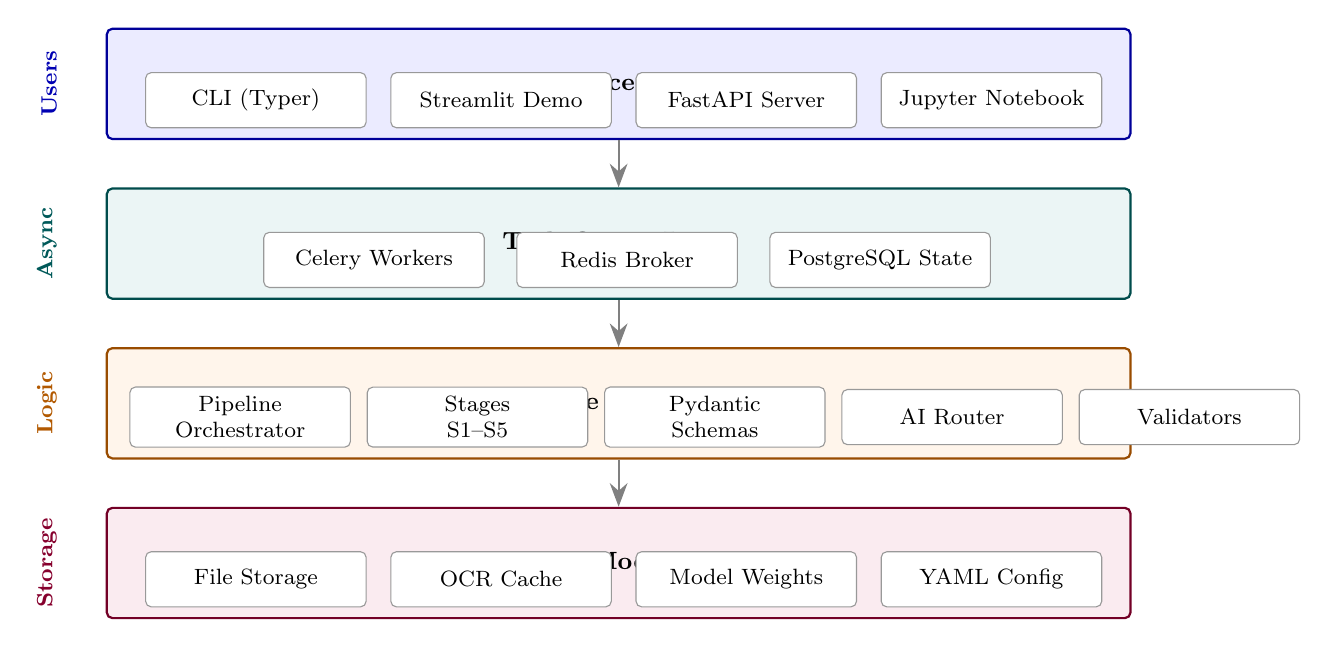
\begin{tikzpicture}[
    node distance=0.5cm,
    layer/.style={
        rectangle, rounded corners=2pt, draw=#1!60!black, thick,
        minimum width=13cm, minimum height=1.4cm,
        fill=#1!8, font=\small\bfseries, align=center
    },
    component/.style={
        rectangle, rounded corners=2pt, draw=black!40,
        minimum width=2.8cm, minimum height=0.7cm,
        fill=white, font=\footnotesize, align=center
    },
    arrow/.style={-{Stealth[length=3mm]}, thick, draw=black!50},
    layerlabel/.style={font=\footnotesize\bfseries, text=#1!70!black}
]

% Layer 1: Interface
\node[layer=blue] (l1) {Interface Layer};
\node[component, above=0.15cm of l1.south west, anchor=south west, xshift=0.5cm] (cli) {CLI (Typer)};
\node[component, right=0.3cm of cli] (demo) {Streamlit Demo};
\node[component, right=0.3cm of demo] (api) {FastAPI Server};
\node[component, right=0.3cm of api] (notebook) {Jupyter Notebook};

% Layer 2: Task Queue
\node[layer=teal, below=0.6cm of l1] (l2) {Task Queue Layer};
\node[component, above=0.15cm of l2.south west, anchor=south west, xshift=2.0cm] (celery) {Celery Workers};
\node[component, right=0.4cm of celery] (redis) {Redis Broker};
\node[component, right=0.4cm of redis] (pg) {PostgreSQL State};

% Layer 3: Core Engine
\node[layer=orange, below=0.6cm of l2] (l3) {Core Engine (Pure Python)};
\node[component, above=0.15cm of l3.south west, anchor=south west, xshift=0.3cm] (pipeline) {Pipeline\\Orchestrator};
\node[component, right=0.2cm of pipeline] (stages) {Stages\\S1--S5};
\node[component, right=0.2cm of stages] (schemas) {Pydantic\\Schemas};
\node[component, right=0.2cm of schemas] (router) {AI Router};
\node[component, right=0.2cm of router] (validators) {Validators};

% Layer 4: Data
\node[layer=purple, below=0.6cm of l3] (l4) {Data \& Model Layer};
\node[component, above=0.15cm of l4.south west, anchor=south west, xshift=0.5cm] (files) {File Storage};
\node[component, right=0.3cm of files] (cache) {OCR Cache};
\node[component, right=0.3cm of cache] (weights) {Model Weights};
\node[component, right=0.3cm of weights] (config) {YAML Config};

% Arrows
\draw[arrow] (l1) -- (l2);
\draw[arrow] (l2) -- (l3);
\draw[arrow] (l3) -- (l4);

% Side labels
\node[layerlabel=blue, rotate=90, anchor=south] at ($(l1.west) + (-0.5, 0)$) {Users};
\node[layerlabel=teal, rotate=90, anchor=south] at ($(l2.west) + (-0.5, 0)$) {Async};
\node[layerlabel=orange, rotate=90, anchor=south] at ($(l3.west) + (-0.5, 0)$) {Logic};
\node[layerlabel=purple, rotate=90, anchor=south] at ($(l4.west) + (-0.5, 0)$) {Storage};

\end{tikzpicture}

% Requires: \usepackage{tikz} \usetikzlibrary{shapes.geometric, arrows.meta, positioning, fit, backgrounds, calc}

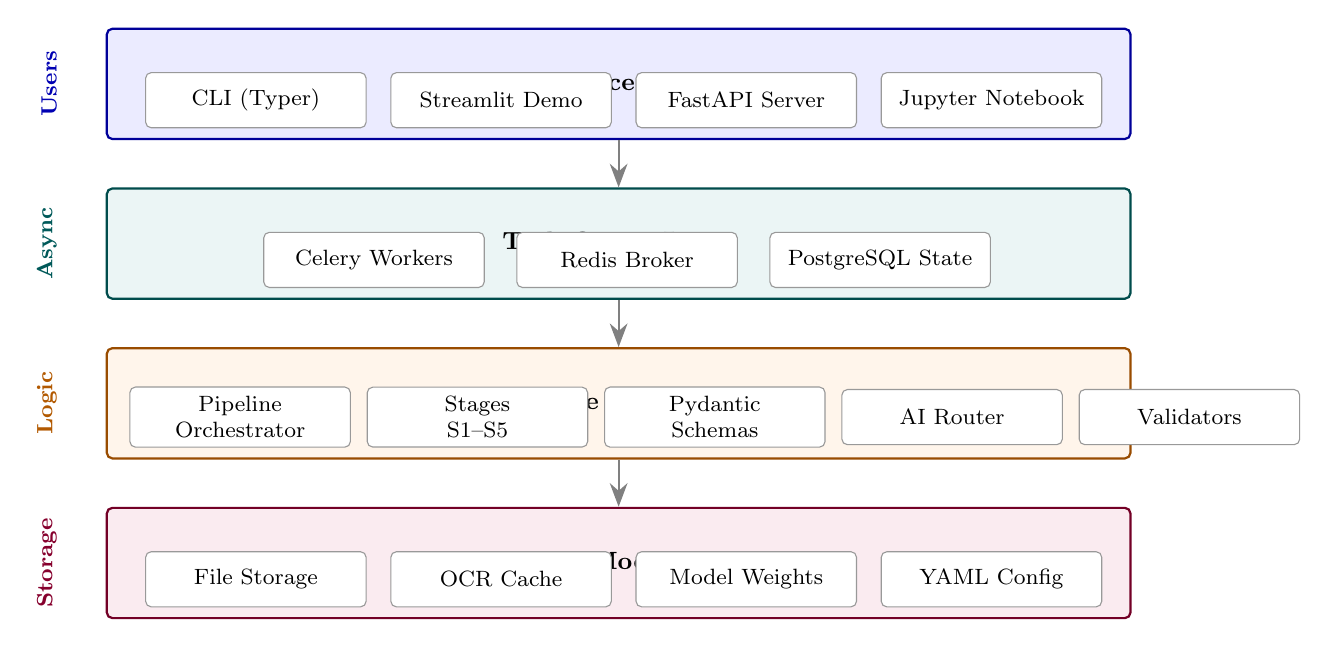
\begin{tikzpicture}[
    node distance=0.5cm,
    layer/.style={
        rectangle, rounded corners=2pt, draw=#1!60!black, thick,
        minimum width=13cm, minimum height=1.4cm,
        fill=#1!8, font=\small\bfseries, align=center
    },
    component/.style={
        rectangle, rounded corners=2pt, draw=black!40,
        minimum width=2.8cm, minimum height=0.7cm,
        fill=white, font=\footnotesize, align=center
    },
    arrow/.style={-{Stealth[length=3mm]}, thick, draw=black!50},
    layerlabel/.style={font=\footnotesize\bfseries, text=#1!70!black}
]

% Layer 1: Interface
\node[layer=blue] (l1) {Interface Layer};
\node[component, above=0.15cm of l1.south west, anchor=south west, xshift=0.5cm] (cli) {CLI (Typer)};
\node[component, right=0.3cm of cli] (demo) {Streamlit Demo};
\node[component, right=0.3cm of demo] (api) {FastAPI Server};
\node[component, right=0.3cm of api] (notebook) {Jupyter Notebook};

% Layer 2: Task Queue
\node[layer=teal, below=0.6cm of l1] (l2) {Task Queue Layer};
\node[component, above=0.15cm of l2.south west, anchor=south west, xshift=2.0cm] (celery) {Celery Workers};
\node[component, right=0.4cm of celery] (redis) {Redis Broker};
\node[component, right=0.4cm of redis] (pg) {PostgreSQL State};

% Layer 3: Core Engine
\node[layer=orange, below=0.6cm of l2] (l3) {Core Engine (Pure Python)};
\node[component, above=0.15cm of l3.south west, anchor=south west, xshift=0.3cm] (pipeline) {Pipeline\\Orchestrator};
\node[component, right=0.2cm of pipeline] (stages) {Stages\\S1--S5};
\node[component, right=0.2cm of stages] (schemas) {Pydantic\\Schemas};
\node[component, right=0.2cm of schemas] (router) {AI Router};
\node[component, right=0.2cm of router] (validators) {Validators};

% Layer 4: Data
\node[layer=purple, below=0.6cm of l3] (l4) {Data \& Model Layer};
\node[component, above=0.15cm of l4.south west, anchor=south west, xshift=0.5cm] (files) {File Storage};
\node[component, right=0.3cm of files] (cache) {OCR Cache};
\node[component, right=0.3cm of cache] (weights) {Model Weights};
\node[component, right=0.3cm of weights] (config) {YAML Config};

% Arrows
\draw[arrow] (l1) -- (l2);
\draw[arrow] (l2) -- (l3);
\draw[arrow] (l3) -- (l4);

% Side labels
\node[layerlabel=blue, rotate=90, anchor=south] at ($(l1.west) + (-0.5, 0)$) {Users};
\node[layerlabel=teal, rotate=90, anchor=south] at ($(l2.west) + (-0.5, 0)$) {Async};
\node[layerlabel=orange, rotate=90, anchor=south] at ($(l3.west) + (-0.5, 0)$) {Logic};
\node[layerlabel=purple, rotate=90, anchor=south] at ($(l4.west) + (-0.5, 0)$) {Storage};

\end{tikzpicture}

\caption{Geo-SLM 5-layer system architecture. Each layer depends only on layers below it.
    The Core Engine is independent of the serving layer.}
\label{fig:layer_arch}
\end{figure}

\Cref{tab:tech} lists the technology stack for each component.

\begin{table}[htbp]
\centering
\caption{Technology stack overview.}
\label{tab:tech}
\begin{table}[htbp]
\centering
\caption{Core Technology Stack}
\label{tab:technology-stack}
\begin{tabular}{@{}llp{5cm}@{}}
\toprule
\textbf{Component} & \textbf{Technology} & \textbf{Rationale} \\
\midrule
Language         & Python 3.11+          & AI/ML ecosystem maturity \\
Object Detection & YOLOv8m (Ultralytics) & Fast, accurate, trainable \\
OCR              & EasyOCR / PaddleOCR   & Multi-language support \\
Image Processing & OpenCV + Pillow       & Industry standard \\
Geometric Calc.  & NumPy + Custom        & Precision arithmetic \\
Classification   & ResNet-18 (PyTorch)   & Lightweight, 94.14\% accuracy \\
Data Validation  & Pydantic v2           & Runtime schema enforcement \\
Configuration    & OmegaConf (YAML)      & Hierarchical ML config \\
\bottomrule
\end{tabular}
\end{table}
\end{table}

% ============================================================
\subsection{Stage 1: Ingestion and Sanitation}
% ============================================================

Stage~1 transforms diverse input formats (PDF, PNG, JPG, TIFF, BMP) into normalized
\texttt{CleanImage} objects. Key operations include:

\begin{itemize}
    \item \textbf{PDF rendering}: PyMuPDF renders each page using a transformation matrix
          \texttt{Matrix(DPI/72, DPI/72)} at a configurable DPI (default: 150).
    \item \textbf{Quality validation}: Blur detection using Laplacian variance
          ($\sigma^2(\nabla^2 I)$); images below the threshold (100.0) are flagged but
          not rejected, deferring the decision to downstream stages.
    \item \textbf{Normalization}: Images exceeding 4,096 pixels are downscaled with
          \texttt{INTER\_AREA} interpolation; images below 100 pixels are rejected.
    \item \textbf{Session management}: Each pipeline run generates a unique session ID
          (\texttt{sess\_YYYYMMDD\_HHMMSS\_\{uuid8\}}) and a config hash for
          reproducibility.
\end{itemize}

Stage~1 is marked as \emph{critical} -- the pipeline cannot proceed without valid input.
If ingestion fails, a \texttt{StageInputError} is raised rather than producing an
empty output.

% ============================================================
\subsection{Stage 2: Detection and Localization}
% ============================================================

Stage~2 detects chart regions in document images using a trained YOLOv8m model
\cite{jocher2023yolov8}. The detection pipeline operates as follows:

\begin{enumerate}
    \item Load each \texttt{CleanImage} and run YOLO inference (confidence threshold 0.5,
          NMS IoU threshold 0.45, input size $640 \times 640$).
    \item Filter detections by minimum area (100~pixels).
    \item For each valid detection, crop the chart region with 10-pixel padding to prevent
          text clipping, assign a unique \texttt{chart\_id}, and save the cropped image.
\end{enumerate}

The detector uses a \textbf{single-class strategy} (``chart'' vs.\ background) rather
than multi-class per chart type. This design decision is motivated by the observation
that YOLO excels at localization, while type classification benefits from a dedicated
architecture (ResNet-18, see \Cref{sec:system_s3}). The two-model cascade achieves
higher combined accuracy than a single multi-class detector.

Training uses conservative augmentation (no rotation or flipping, since charts are
orientation-sensitive) with mosaic, scale, HSV adjustments, and translation.

% ============================================================
\subsection{Stage 3: Structural Analysis (Extraction)}
\label{sec:system_s3}
% ============================================================

Stage~3 is the most complex component ($\sim$5,400 lines across 7 submodules). Its core
design principle is to treat charts as \textbf{collections of geometric entities} rather
than pixel patterns. \Cref{fig:s3_submodules} shows the submodule pipeline.

\begin{figure}[htbp]
\centering
% TikZ: Stage 3 Extraction Submodules
% Usage: % TikZ: Stage 3 Extraction Submodules
% Usage: \input{figures/tikz/tikz_stage3_submodules.tex}
% Requires: \usepackage{tikz} \usetikzlibrary{shapes.geometric, arrows.meta, positioning, fit, backgrounds}

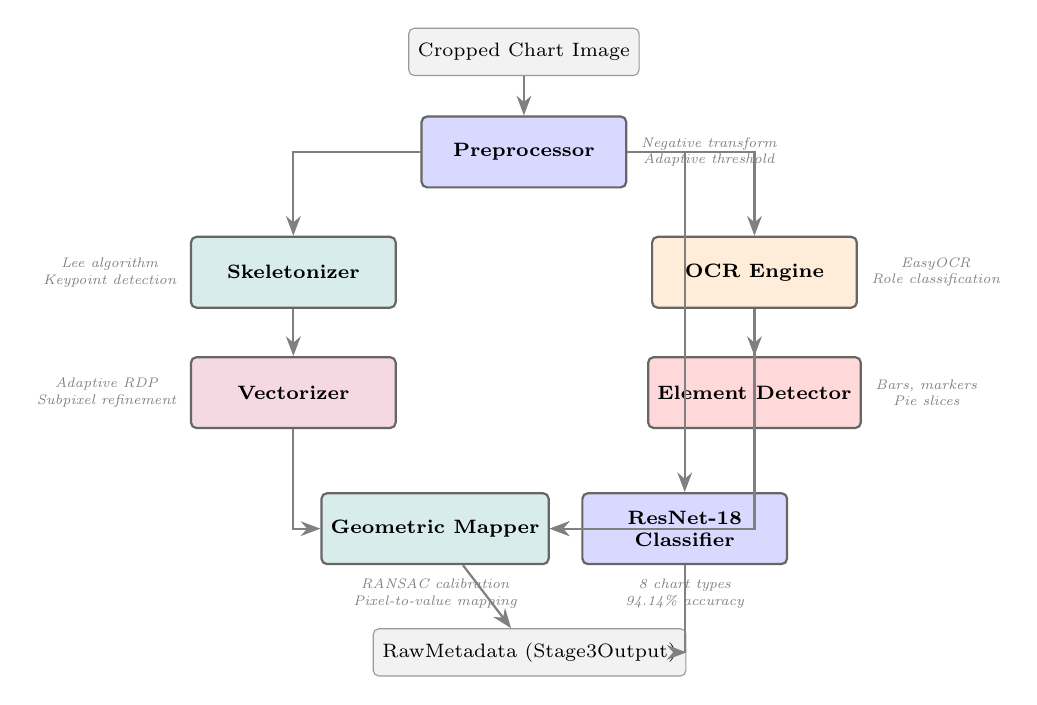
\begin{tikzpicture}[
    node distance=0.4cm and 0.3cm,
    module/.style={
        rectangle, rounded corners=2pt, draw=black!60, thick,
        minimum width=2.6cm, minimum height=0.9cm,
        fill=#1!15, font=\scriptsize\bfseries, align=center
    },
    arrow/.style={-{Stealth[length=2.5mm]}, thick, draw=black!50},
    label/.style={font=\tiny\itshape, text=black!50, align=center},
    io/.style={
        rectangle, rounded corners=2pt, draw=black!40,
        minimum width=2.2cm, minimum height=0.6cm,
        fill=black!5, font=\scriptsize, align=center
    }
]

% Input
\node[io] (input) {Cropped Chart Image};

% Row 1: Preprocessing
\node[module=blue, below=0.5cm of input] (prep) {Preprocessor};
\node[label, right=0.05cm of prep] {Negative transform\\Adaptive threshold};

% Row 2: Skeleton + OCR (parallel)
\node[module=teal, below left=0.6cm and 0.3cm of prep] (skel) {Skeletonizer};
\node[module=orange, below right=0.6cm and 0.3cm of prep] (ocr) {OCR Engine};
\node[label, left=0.05cm of skel] {Lee algorithm\\Keypoint detection};
\node[label, right=0.05cm of ocr] {EasyOCR\\Role classification};

% Row 3: Vectorizer + Elements
\node[module=purple, below=0.6cm of skel] (vec) {Vectorizer};
\node[module=red, below=0.6cm of ocr] (elem) {Element Detector};
\node[label, left=0.05cm of vec] {Adaptive RDP\\Subpixel refinement};
\node[label, right=0.05cm of elem] {Bars, markers\\Pie slices};

% Row 4: Geometric Mapper + Classifier (merge)
\node[module=teal, below=0.8cm of vec, xshift=1.8cm] (geo) {Geometric Mapper};
\node[module=blue, right=0.4cm of geo] (cls) {ResNet-18\\Classifier};
\node[label, below=0.05cm of geo] {RANSAC calibration\\Pixel-to-value mapping};
\node[label, below=0.05cm of cls] {8 chart types\\94.14\% accuracy};

% Output
\node[io, below=0.8cm of geo, xshift=1.2cm] (output) {RawMetadata (Stage3Output)};

% Arrows
\draw[arrow] (input) -- (prep);
\draw[arrow] (prep) -| (skel);
\draw[arrow] (prep) -| (ocr);
\draw[arrow] (skel) -- (vec);
\draw[arrow] (ocr) -- (elem);
\draw[arrow] (vec) |- (geo);
\draw[arrow] (elem) |- (geo);
\draw[arrow] (ocr) |- (geo);
\draw[arrow] (prep) -| (cls);
\draw[arrow] (geo) -- (output);
\draw[arrow] (cls) |- (output);

\end{tikzpicture}

% Requires: \usepackage{tikz} \usetikzlibrary{shapes.geometric, arrows.meta, positioning, fit, backgrounds}

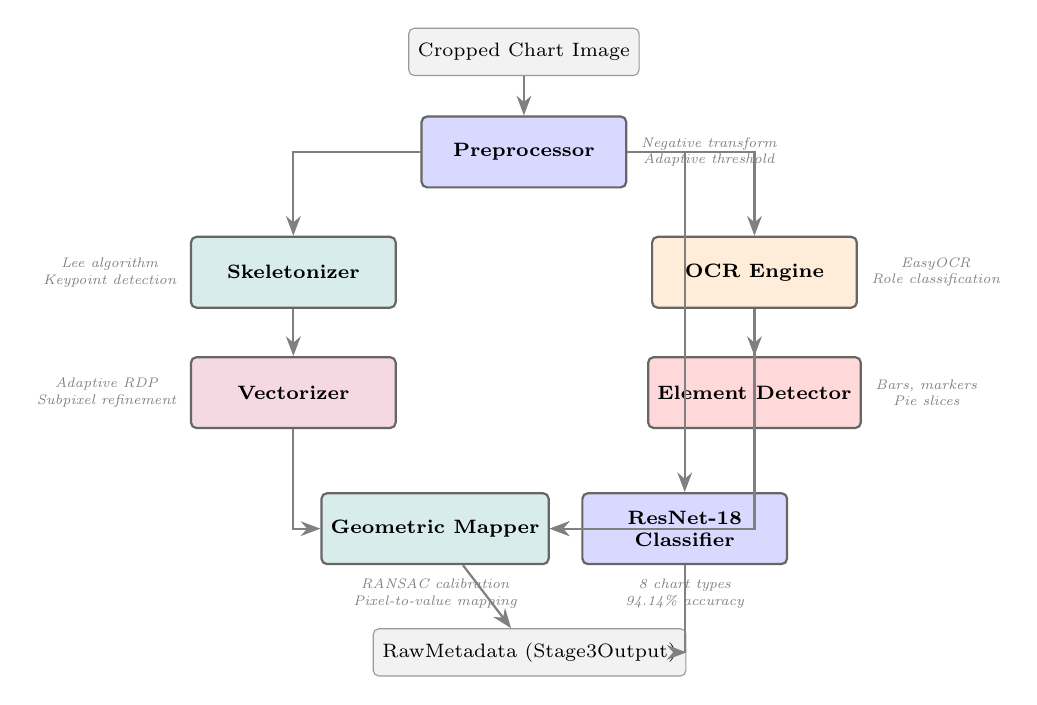
\begin{tikzpicture}[
    node distance=0.4cm and 0.3cm,
    module/.style={
        rectangle, rounded corners=2pt, draw=black!60, thick,
        minimum width=2.6cm, minimum height=0.9cm,
        fill=#1!15, font=\scriptsize\bfseries, align=center
    },
    arrow/.style={-{Stealth[length=2.5mm]}, thick, draw=black!50},
    label/.style={font=\tiny\itshape, text=black!50, align=center},
    io/.style={
        rectangle, rounded corners=2pt, draw=black!40,
        minimum width=2.2cm, minimum height=0.6cm,
        fill=black!5, font=\scriptsize, align=center
    }
]

% Input
\node[io] (input) {Cropped Chart Image};

% Row 1: Preprocessing
\node[module=blue, below=0.5cm of input] (prep) {Preprocessor};
\node[label, right=0.05cm of prep] {Negative transform\\Adaptive threshold};

% Row 2: Skeleton + OCR (parallel)
\node[module=teal, below left=0.6cm and 0.3cm of prep] (skel) {Skeletonizer};
\node[module=orange, below right=0.6cm and 0.3cm of prep] (ocr) {OCR Engine};
\node[label, left=0.05cm of skel] {Lee algorithm\\Keypoint detection};
\node[label, right=0.05cm of ocr] {EasyOCR\\Role classification};

% Row 3: Vectorizer + Elements
\node[module=purple, below=0.6cm of skel] (vec) {Vectorizer};
\node[module=red, below=0.6cm of ocr] (elem) {Element Detector};
\node[label, left=0.05cm of vec] {Adaptive RDP\\Subpixel refinement};
\node[label, right=0.05cm of elem] {Bars, markers\\Pie slices};

% Row 4: Geometric Mapper + Classifier (merge)
\node[module=teal, below=0.8cm of vec, xshift=1.8cm] (geo) {Geometric Mapper};
\node[module=blue, right=0.4cm of geo] (cls) {ResNet-18\\Classifier};
\node[label, below=0.05cm of geo] {RANSAC calibration\\Pixel-to-value mapping};
\node[label, below=0.05cm of cls] {8 chart types\\94.14\% accuracy};

% Output
\node[io, below=0.8cm of geo, xshift=1.2cm] (output) {RawMetadata (Stage3Output)};

% Arrows
\draw[arrow] (input) -- (prep);
\draw[arrow] (prep) -| (skel);
\draw[arrow] (prep) -| (ocr);
\draw[arrow] (skel) -- (vec);
\draw[arrow] (ocr) -- (elem);
\draw[arrow] (vec) |- (geo);
\draw[arrow] (elem) |- (geo);
\draw[arrow] (ocr) |- (geo);
\draw[arrow] (prep) -| (cls);
\draw[arrow] (geo) -- (output);
\draw[arrow] (cls) |- (output);

\end{tikzpicture}

\caption{Stage~3 extraction pipeline: 7 submodules process the cropped chart image
    sequentially. Each submodule has an independent configuration and can be toggled on/off.}
\label{fig:s3_submodules}
\end{figure}

\subsubsection{Preprocessor}

The preprocessor converts chart images to optimized binary masks. A key technique is the
\textbf{negative image transform}: $I_{\text{neg}} = 255 - I$. This inversion aligns
chart strokes (thin, dark lines) with morphological operations that expect bright
foreground, improving skeleton quality by approximately 30\%. Adaptive Gaussian
thresholding ($T(x,y) = \mu_G(x,y) - C$, block size 11, $C=2$) handles non-uniform
lighting in scanned documents.

\subsubsection{Skeletonizer}

The Lee topology-preserving thinning algorithm \cite{lee1994skeleton} reduces thick
strokes to 1-pixel width while maintaining 8-connectivity and homotopy (no holes or
junctions are created or destroyed). Gap filling via morphological closing
(\texttt{kernel=3$\times$3}) precedes skeletonization to repair small breaks in chart
lines. Junction detection classifies skeleton pixels as endpoints (1~neighbor),
junctions (3+ neighbors), or intermediate (2~neighbors).

\subsubsection{Vectorizer}

The Ramer-Douglas-Peucker (RDP) algorithm \cite{douglas1973rdp, ramer1972rdp}
recursively simplifies polylines by removing points within tolerance $\epsilon$.
Geo-SLM uses an \textbf{adaptive epsilon}:
\begin{equation}
    \epsilon = \epsilon_{\text{base}} \cdot \sqrt{\frac{L}{L_{\text{ref}}}}
\end{equation}
where $L$ is the polyline length and $L_{\text{ref}}$ is a reference length. This
prevents over-simplification of long curves and under-simplification of short ones.
Sub-pixel refinement uses weighted centroids for fractional pixel positions.

\subsubsection{OCR Engine}

PaddleOCR \cite{du2020paddleocr} (with EasyOCR \cite{jaided2020easyocr} as fallback)
extracts all text, which is then assigned spatial roles based on position: title
(top 15\%), X-axis label (bottom 15\%), Y-axis label (left 15\%), legend
(top-right corner), and data values (near elements). Content-aware keyword matching
supplements positional heuristics.

\subsubsection{Element Detector}

Three detection methods are combined for bar detection: watershed segmentation for
touching bars, projection profile analysis for alignment, and morphological connected
components. Scatter plot markers use Hough circle transform. Pie slices use contour
analysis with arc fitting. Color clustering (K-means, $k=8$) identifies dominant
colors per element.

\subsubsection{Geometric Mapper}

The geometric mapper calibrates axes and converts pixel coordinates to data values.
The calibration pipeline:

\begin{enumerate}
    \item Match OCR tick labels to detected tick positions along axes.
    \item Build (pixel, value) correspondence pairs.
    \item Fit a calibration model using RANSAC \cite{fischler1981ransac} (default),
          which tolerates up to 40\% outlier rejection from OCR errors.
    \item Compute $R^2$ as calibration confidence.
\end{enumerate}

The linear mapping function (with Y-axis inversion for image coordinates):
\begin{equation}
    v_y = y_{\max} - \frac{p_y - p_{\text{top}}}{p_{\text{bottom}} - p_{\text{top}}}
          \cdot (y_{\max} - y_{\min})
\end{equation}
Logarithmic scale is detected automatically when tick values follow a geometric
progression.

\subsubsection{Classifier}

A cascade of three classifiers determines chart type:

\begin{enumerate}
    \item \textbf{ResNet-18} \cite{he2016resnet}: CNN on $256 \times 256$ grayscale input,
          8 classes, 94.14\% test accuracy, 6.90ms ONNX inference (CPU).
    \item \textbf{ML Classifier}: Random Forest on structural features ($\sim$70\% accuracy).
    \item \textbf{Rule-based}: Heuristics (has bars? has slices?) as final fallback
          ($\sim$50\% accuracy).
\end{enumerate}

The overall extraction confidence is a weighted average:
\begin{equation}
    C_{\text{overall}} = 0.3 \cdot C_{\text{class}} + 0.25 \cdot C_{\text{ocr}}
                       + 0.25 \cdot C_{\text{axis}} + 0.2 \cdot C_{\text{elem}}
\end{equation}

% ============================================================
\subsection{Stage 4: Semantic Reasoning}
% ============================================================

Stage~4 refines raw extracted metadata using AI reasoning. The processing pipeline
per chart consists of four steps:

\textbf{Step 1: Geometric Value Mapping.}
The \texttt{GeometricValueMapper} (764 lines) applies the calibration from Stage~3 to
convert all pixel coordinates to data values. Confidence filtering ensures mapping is
applied only when calibration confidence $\geq 0.3$. Value clamping restricts results
to the detected axis range to prevent extrapolation errors.

\textbf{Step 2: Prompt Construction.}
The \texttt{GeminiPromptBuilder} (833 lines) constructs structured prompts with explicit
sections: \textsc{Chart\_Metadata}, \textsc{OCR\_Texts}, \textsc{Elements},
\textsc{Axis\_Info}, \textsc{Mapped\_Values}, and \textsc{Instructions}. Anti-hallucination
rules are embedded: ``Only report values that appear in OCR\_TEXTS or MAPPED\_VALUES;
if uncertain, report null rather than guess.''

\textbf{Step 3: AI Routing.}
The \texttt{AIRouterEngine} delegates to the AI Router (see \Cref{sec:ai_routing}).
The router walks the task-specific fallback chain until a provider returns a response
with confidence above threshold (0.7).

\textbf{Step 4: Post-processing.}
The AI response is parsed into structured \texttt{RefinedChartData}: title, axis labels,
named data series with $(x, y)$ points, natural language description, and confidence
scores.

A pure rule-based fallback is available when all AI providers fail, applying pattern-based
OCR corrections and direct use of geometric mapping values without LLM refinement.

% ============================================================
\subsection{Stage 5: Insight and Reporting}
% ============================================================

Stage~5 generates human-readable insights from structured chart data and produces
final output files. Four insight types are supported:

\begin{itemize}
    \item \textbf{Trend detection}: Linear regression slope classification
          (increasing, decreasing, stable, volatile), with $R^2$ as confidence.
    \item \textbf{Comparison}: Cross-series analysis (dominant series, largest gap,
          crossover points) for charts with $\geq 2$ data series.
    \item \textbf{Anomaly detection}: Z-score method ($|z| > 2.0$) applied per-series.
    \item \textbf{Summary}: Template-based text combining chart type, axis labels,
          data range, and trend information.
\end{itemize}

Output is produced in two formats: (1) a structured JSON file containing the full
\texttt{PipelineResult} with session metadata, all chart results, insights, and
source traceability; and (2) a Markdown report with per-chart sections. Failed charts
are included with error insights rather than dropped, preserving pipeline completeness.

% ============================================================
\subsection{AI Routing Layer}
\label{sec:ai_routing}
% ============================================================

\Cref{fig:ai_router} illustrates the AI routing architecture.

\begin{figure}[htbp]
\centering
% TikZ: AI Router with Fallback Chains
% Usage: % TikZ: AI Router with Fallback Chains
% Usage: \input{figures/tikz/tikz_ai_router.tex}
% Requires: \usepackage{tikz} \usetikzlibrary{shapes.geometric, arrows.meta, positioning, fit, backgrounds, calc}

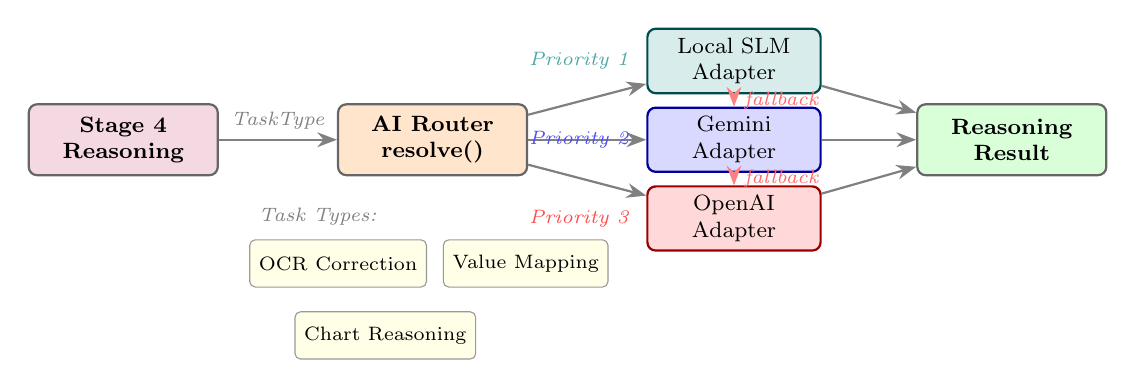
\begin{tikzpicture}[
    node distance=0.6cm and 0.8cm,
    block/.style={
        rectangle, rounded corners=3pt, draw=black!60, thick,
        minimum width=2.4cm, minimum height=0.9cm,
        font=\footnotesize\bfseries, align=center
    },
    adapter/.style={
        rectangle, rounded corners=3pt, draw=#1!60!black, thick,
        minimum width=2.2cm, minimum height=0.8cm,
        fill=#1!15, font=\footnotesize, align=center
    },
    task/.style={
        rectangle, rounded corners=2pt, draw=black!40,
        minimum width=2.0cm, minimum height=0.6cm,
        fill=yellow!10, font=\scriptsize, align=center
    },
    arrow/.style={-{Stealth[length=2.5mm]}, thick, draw=black!50},
    dasharrow/.style={-{Stealth[length=2.5mm]}, dashed, draw=red!50, thick},
    label/.style={font=\scriptsize\itshape, text=black!50}
]

% Stage 4 caller
\node[block, fill=purple!15] (caller) {Stage 4\\Reasoning};

% Router
\node[block, fill=orange!20, right=1.5cm of caller] (router) {AI Router\\resolve()};

% Adapters
\node[adapter=teal, right=1.5cm of router, yshift=1.0cm] (slm) {Local SLM\\Adapter};
\node[adapter=blue, right=1.5cm of router] (gemini) {Gemini\\Adapter};
\node[adapter=red, right=1.5cm of router, yshift=-1.0cm] (openai) {OpenAI\\Adapter};

% Standardized output
\node[block, fill=green!15, right=1.2cm of gemini] (result) {Reasoning\\Result};

% Arrows: caller -> router
\draw[arrow] (caller) -- node[above, label] {TaskType} (router);

% Router -> adapters
\draw[arrow] (router) -- (slm);
\draw[arrow] (router) -- (gemini);
\draw[arrow] (router) -- (openai);

% Adapters -> result
\draw[arrow] (slm) -- (result);
\draw[arrow] (gemini) -- (result);
\draw[arrow] (openai) -- (result);

% Fallback arrows
\draw[dasharrow] (slm.south) -- node[right, label, text=red!60] {fallback} (gemini.north);
\draw[dasharrow] (gemini.south) -- node[right, label, text=red!60] {fallback} (openai.north);

% Task type examples below router
\node[task, below=0.8cm of router, xshift=-1.2cm] (t1) {OCR Correction};
\node[task, right=0.2cm of t1] (t2) {Value Mapping};
\node[task, below=0.3cm of t1, xshift=0.6cm] (t3) {Chart Reasoning};

\node[label, above=0.05cm of t1.north west, anchor=south west] {Task Types:};

% Priority labels
\node[label, left=0.1cm of slm, text=teal!70] {Priority 1};
\node[label, left=0.1cm of gemini, text=blue!70] {Priority 2};
\node[label, left=0.1cm of openai, text=red!70] {Priority 3};

\end{tikzpicture}

% Requires: \usepackage{tikz} \usetikzlibrary{shapes.geometric, arrows.meta, positioning, fit, backgrounds, calc}

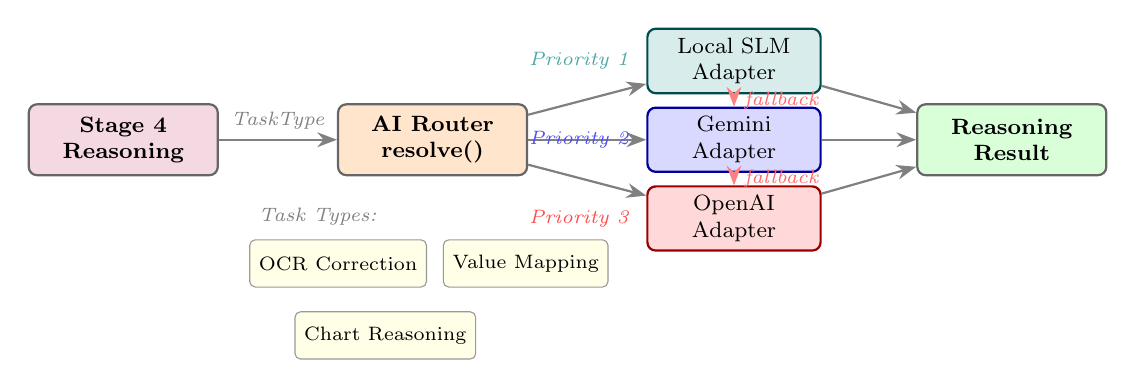
\begin{tikzpicture}[
    node distance=0.6cm and 0.8cm,
    block/.style={
        rectangle, rounded corners=3pt, draw=black!60, thick,
        minimum width=2.4cm, minimum height=0.9cm,
        font=\footnotesize\bfseries, align=center
    },
    adapter/.style={
        rectangle, rounded corners=3pt, draw=#1!60!black, thick,
        minimum width=2.2cm, minimum height=0.8cm,
        fill=#1!15, font=\footnotesize, align=center
    },
    task/.style={
        rectangle, rounded corners=2pt, draw=black!40,
        minimum width=2.0cm, minimum height=0.6cm,
        fill=yellow!10, font=\scriptsize, align=center
    },
    arrow/.style={-{Stealth[length=2.5mm]}, thick, draw=black!50},
    dasharrow/.style={-{Stealth[length=2.5mm]}, dashed, draw=red!50, thick},
    label/.style={font=\scriptsize\itshape, text=black!50}
]

% Stage 4 caller
\node[block, fill=purple!15] (caller) {Stage 4\\Reasoning};

% Router
\node[block, fill=orange!20, right=1.5cm of caller] (router) {AI Router\\resolve()};

% Adapters
\node[adapter=teal, right=1.5cm of router, yshift=1.0cm] (slm) {Local SLM\\Adapter};
\node[adapter=blue, right=1.5cm of router] (gemini) {Gemini\\Adapter};
\node[adapter=red, right=1.5cm of router, yshift=-1.0cm] (openai) {OpenAI\\Adapter};

% Standardized output
\node[block, fill=green!15, right=1.2cm of gemini] (result) {Reasoning\\Result};

% Arrows: caller -> router
\draw[arrow] (caller) -- node[above, label] {TaskType} (router);

% Router -> adapters
\draw[arrow] (router) -- (slm);
\draw[arrow] (router) -- (gemini);
\draw[arrow] (router) -- (openai);

% Adapters -> result
\draw[arrow] (slm) -- (result);
\draw[arrow] (gemini) -- (result);
\draw[arrow] (openai) -- (result);

% Fallback arrows
\draw[dasharrow] (slm.south) -- node[right, label, text=red!60] {fallback} (gemini.north);
\draw[dasharrow] (gemini.south) -- node[right, label, text=red!60] {fallback} (openai.north);

% Task type examples below router
\node[task, below=0.8cm of router, xshift=-1.2cm] (t1) {OCR Correction};
\node[task, right=0.2cm of t1] (t2) {Value Mapping};
\node[task, below=0.3cm of t1, xshift=0.6cm] (t3) {Chart Reasoning};

\node[label, above=0.05cm of t1.north west, anchor=south west] {Task Types:};

% Priority labels
\node[label, left=0.1cm of slm, text=teal!70] {Priority 1};
\node[label, left=0.1cm of gemini, text=blue!70] {Priority 2};
\node[label, left=0.1cm of openai, text=red!70] {Priority 3};

\end{tikzpicture}

\caption{AI Router with Adapter Pattern and per-task fallback chains.
    Each provider implements the common \texttt{BaseAIAdapter} interface.}
\label{fig:ai_router}
\end{figure}

All AI providers implement \texttt{BaseAIAdapter}, an abstract base class defining
\texttt{reason()}, \texttt{correct\_ocr()}, and \texttt{health\_check()} methods.
Concrete adapters (\texttt{GeminiAdapter}, \texttt{OpenAIAdapter},
\texttt{LocalSLMAdapter}) handle provider-specific API calls, authentication, and
error wrapping.

\Cref{tab:ai_providers} shows the configured providers and their roles.

\begin{table}[htbp]
\centering
\caption{AI provider configuration.}
\label{tab:ai_providers}
\begin{tabular}{@{}lllll@{}}
\toprule
\textbf{Provider} & \textbf{Model} & \textbf{Use Case} & \textbf{Priority} & \textbf{Cost} \\
\midrule
Local SLM & Qwen-2.5-1.5B    & Default reasoning   & Primary    & Free \\
Gemini    & gemini-2.0-flash  & Complex charts       & Fallback 1 & API \\
OpenAI    & gpt-4o-mini       & Alternative          & Fallback 2 & API \\
\bottomrule
\end{tabular}
\end{table}

The \texttt{AIRouter} resolves a (adapter, model\_id) pair for each task type by:
(1)~checking configuration overrides, (2)~walking the fallback chain for the task type,
(3)~verifying API key availability and provider health, and (4)~returning the first
healthy provider. A \textbf{local-only mode} restricts routing to the local SLM for
privacy-sensitive or offline deployments.

% ============================================================
\subsection{Error Handling and Extensibility}
% ============================================================

The system uses a hierarchical exception system rooted at \texttt{ChartAnalysisError}.
Each exception carries \texttt{stage}, \texttt{recoverable}, and
\texttt{fallback\_available} flags, enabling the orchestrator to decide whether to
continue, retry, or abort.

The modular architecture provides five extension points:
\begin{itemize}
    \item \textbf{New chart type}: Add an enum value to \texttt{ChartType} and element
          detection rules.
    \item \textbf{New AI provider}: Implement \texttt{BaseAIAdapter} and register in the
          router configuration.
    \item \textbf{New pipeline stage}: Implement \texttt{BaseStage[In, Out]} and register
          in the orchestrator.
    \item \textbf{New output format}: Add to \texttt{OutputFormat} enum and write a
          formatter in Stage~5.
    \item \textbf{New language}: Change OCR config, add keyword dictionaries, create
          prompt template variants, and fine-tune SLM with target-language data --
          all without modifying core pipeline logic.
    \item \textbf{Configuration override}: Add a YAML key; OmegaConf handles hierarchical
          merging.
\end{itemize}

% ============================================================
\subsection{Vietnamese Language Implementation}
\label{sec:viet_impl}
% ============================================================

This subsection details the concrete implementation path for Vietnamese chart
understanding, demonstrating how the extension module architecture supports language
localization at each pipeline stage.

\subsubsection{Language-Agnostic vs.\ Language-Dependent Components}

\Cref{tab:lang_analysis} classifies each pipeline component by its language dependency.
The classification reveals that the majority of the system -- the entire geometric
analysis core -- is inherently language-agnostic.

\begin{table}[htbp]
\centering
\caption{Language dependency analysis of pipeline components.}
\label{tab:lang_analysis}
\begin{tabular}{@{}lllp{5.5cm}@{}}
\toprule
\textbf{Component} & \textbf{Stage} & \textbf{Language Dep.} & \textbf{Rationale} \\
\midrule
PDF Renderer           & S1 & Agnostic  & Pixel-level rendering, no text parsing \\
Blur Detector          & S1 & Agnostic  & Laplacian variance is language-free \\
YOLO Detector          & S2 & Agnostic  & Visual bounding box detection \\
Preprocessor           & S3 & Agnostic  & Negative transform, thresholding \\
Skeletonizer           & S3 & Agnostic  & Topology-preserving thinning \\
Vectorizer (RDP)       & S3 & Agnostic  & Polyline simplification \\
Element Detector       & S3 & Agnostic  & Watershed, Hough, contour analysis \\
Geometric Mapper       & S3 & Agnostic  & Pixel-to-value calibration (numeric) \\
ResNet-18 Classifier   & S3 & Agnostic  & Visual feature classification \\
\midrule
OCR Engine             & S3 & \textbf{Config}    & Language set via \texttt{config/models.yaml} \\
OCR Role Classifier    & S3 & \textbf{Keywords}  & English keyword lists, needs Vietnamese extension \\
Prompt Builder         & S4 & \textbf{Templates} & English prompts, needs Vietnamese variants \\
AI Adapters            & S4 & Agnostic  & Pass-through interface, language in prompts \\
AI Router              & S4 & Agnostic  & Provider selection, language-transparent \\
Insight Generator      & S5 & \textbf{Templates} & English summary templates \\
QA Generator           & Data & \textbf{Prompts}   & English generation instructions \\
\bottomrule
\end{tabular}
\end{table}

Out of 17 major components, only 4 require modification (OCR role classifier, prompt
builder, insight generator, QA generator) and 1 requires configuration change (OCR
engine). The remaining 12 components, including all geometric analysis modules, are
fully language-agnostic.

\subsubsection{OCR Engine: Vietnamese Configuration Path}

The \texttt{OCRConfig} class defines a \texttt{languages} parameter (default:
\texttt{["en"]}). Vietnamese support is activated through configuration without code
changes:

\begin{verbatim}
# config/models.yaml -- Vietnamese configuration
ocr:
  paddleocr:
    lang: "vi"          # Vietnamese recognition weights
  easyocr:
    languages: ["vi"]   # Multi-language support
  tesseract:
    lang: "vie"         # Tesseract Vietnamese tessdata
\end{verbatim}

The OCR engine initialization code (\texttt{ocr\_engine.py}) already supports this:
PaddleOCR passes \texttt{lang=self.config.languages[0]}, and EasyOCR passes the full
language list to \texttt{easyocr.Reader()}. For bilingual charts (mixed English and
Vietnamese), the configuration \texttt{["en", "vi"]} enables simultaneous recognition.

\subsubsection{Stage 3: Bilingual Role Classification}

The \texttt{\_classify\_role()} method in the OCR engine uses keyword dictionaries for
semantic role assignment. The Vietnamese extension adds parallel dictionaries:

\begin{verbatim}
# Vietnamese axis label keywords (additive extension)
axis_label_keywords_vi = [
    'so luong', 'ty le', 'gia tri', 'doanh thu',
    'thoi gian', 'nam', 'thang', 'ngay',
    'gia', 'chi phi', 'loi nhuan', 'diem so',
    'do chinh xac', 'sai so', 'mat mat',
]

# Vietnamese legend keywords
legend_keywords_vi = [
    'nhom', 'loai', 'phan loai', 'chuoi',
    'huan luyen', 'kiem tra', 'du doan',
    'mo hinh', 'phuong phap', 'thuat toan',
]
\end{verbatim}

The position-based fallback logic (assigning roles based on text position within the
chart image -- top 15\% for titles, bottom 15\% for X-axis, etc.) remains effective
regardless of language, providing a robust baseline when keyword matching fails.

\subsubsection{Stage 4: Vietnamese Prompt Architecture}

The AI adapter interface (\texttt{BaseAIAdapter.reason()}) accepts
\texttt{system\_prompt} and \texttt{user\_prompt} as string parameters, making it
inherently language-transparent. Vietnamese support is implemented entirely at the
prompt layer:

\begin{enumerate}
    \item \textbf{Vietnamese prompt template files}: New files
          \texttt{prompts/reasoning\_vi.txt}, \texttt{description\_vi.txt}, and
          \texttt{ocr\_correction\_vi.txt} contain Vietnamese system instructions with
          Vietnamese chart analysis terminology.
    \item \textbf{Language routing}: The \texttt{PromptConfig.output\_language} field
          (already defined as \texttt{"english"} by default) is wired into the prompt
          selection logic to choose between English and Vietnamese template sets.
    \item \textbf{SLM compatibility}: The Qwen-2.5 model family supports Vietnamese
          natively in its tokenizer, ensuring efficient token usage for Vietnamese text
          generation without excessive subword splitting.
\end{enumerate}

The anti-hallucination constraints (``only report values from OCR\_TEXTS or
MAPPED\_VALUES'') are preserved in Vietnamese prompts, translated to equivalent
Vietnamese instructions to maintain output grounding.

\subsubsection{Data Factory: Vietnamese QA Generation}

The QA generation pipeline in \texttt{tools/data\_factory/} produces training data by
sending chart features to Gemini API with generation instructions. Vietnamese QA
generation requires:

\begin{enumerate}
    \item Rewriting the system prompt in \texttt{qa\_generator.py} to enforce Vietnamese
          output: all questions, answers, and explanations must be in Vietnamese.
    \item Expanding the question taxonomy with Vietnamese-specific terminology covering
          chart analysis concepts (e.g.,
          ``xu hướng tăng/giảm'',
          ``giá trị lớn nhất'',
          ``so sánh giữa các nhóm'').
    \item Targeting 5,000--10,000 Vietnamese QA samples to supplement the existing
          268,799 English samples.
    \item Validating generated data through the existing verification pipeline with
          Vietnamese-aware quality checks.
\end{enumerate}

The combined English + Vietnamese training data enables the SLM to handle both languages,
with the English foundation providing geometric reasoning knowledge and the Vietnamese
data providing language-specific output capability.
\section{Results and Discussion}

This section presents experimental results from each pipeline stage and the end-to-end
system, followed by analysis, comparison with related work, and recommendations.

% ============================================================
\subsection{Results and Analysis}
% ============================================================

\subsubsection{Stage 2: Chart Detection (YOLOv8m)}

The YOLOv8m detector was trained on the chart detection dataset (approximately 32,440
images, single-class ``chart'') for 100 epochs with SGD optimizer (lr=0.01, momentum=0.937).
\Cref{tab:yolo} presents the detection results.

\begin{table}[htbp]
\centering
\caption{YOLOv8m chart detection results.}
\label{tab:yolo}
\begin{table}[htbp]
\centering
\caption{YOLOv8m Chart Detection Results}
\label{tab:yolo-results}
\begin{tabular}{@{}llll@{}}
\toprule
\textbf{Metric} & \textbf{Value} & \textbf{Target} & \textbf{Status} \\
\midrule
mAP@0.5   & 93.5\% & $>$85\% & Exceeded \\
Precision  & $>$90\% & $>$80\% & Exceeded \\
Recall     & $>$90\% & $>$80\% & Exceeded \\
Strategy   & Single-class (``chart'') & -- & -- \\
Input size & 640$\times$640 & -- & -- \\
\bottomrule
\end{tabular}
\end{table}
\end{table}

The detector achieves 93.5\% mAP@0.5, exceeding the target of 85\%. The single-class
strategy simplifies training and avoids category confusion at the detection stage,
delegating type classification to a dedicated model.

\subsubsection{Stage 2b: Chart Type Classification (Ablation Study)}
\label{sec:results_classifier}

An ablation study was conducted comparing two backbone architectures (EfficientNet-B0
and ResNet-18) and two class-scope configurations. Starting from an 8-class baseline
that included a heterogeneous \texttt{others} catch-all, the scope was narrowed to
the three primary chart types targeted by the pipeline: bar, line, and pie.

\Cref{tab:classifier_ablation} summarises the four experimental runs. All models used
the same training protocol: two-phase training (frozen backbone warm-up for 5 epochs,
then full fine-tune), cosine learning rate schedule, weighted cross-entropy with label
smoothing ($\alpha=0.1$), and early stopping with patience~10.

\begin{table}[htbp]
\centering
\caption{Chart classifier ablation: backbone, resolution, and class scope.}
\label{tab:classifier_ablation}
\begin{tabular}{@{}llccccc@{}}
\toprule
\textbf{Run} & \textbf{Backbone} & \textbf{Size} & \textbf{Classes} & \textbf{Accuracy} & \textbf{Macro F1} & \textbf{Epochs} \\
\midrule
v3 (baseline) & EfficientNet-B0 & 160\,px & 4 (w/ \textit{others}) & 84.64\% & 77.52\% & 60       \\
v1            & EfficientNet-B0 & 224\,px & 3                       & \textbf{97.54\%} & \textbf{94.63\%} & 21 \\
v1            & ResNet-18       & 224\,px & 3                       & 95.95\%          & 92.62\%          & 25 \\
\bottomrule
\end{tabular}

\end{table}

The selected production model is EfficientNet-B0 trained on $224 \times 224$ RGB
input (3-class scope), achieving 97.54\% test accuracy and 94.63\% macro F1 after
early convergence at epoch~21. \Cref{tab:classifier_final} presents the per-class
precision, recall, and F1 breakdown for this model.

\begin{table}[htbp]
\centering
\caption{EfficientNet-B0 3-class per-class evaluation (test set, $n=1{,}952$).}
\label{tab:classifier_final}
\begin{tabular}{@{}lrrr@{}}
\toprule
\textbf{Class} & \textbf{Precision} & \textbf{Recall} & \textbf{F1} \\
\midrule
Bar   & 97.05\% & 97.39\% & 97.22\% \\
Line  & 99.21\% & 97.53\% & 98.36\% \\
Pie   & 79.81\% & 98.81\% & 88.30\% \\
\midrule
\textbf{Macro} & \textbf{92.02\%} & \textbf{97.91\%} & \textbf{94.63\%} \\
\bottomrule
\end{tabular}

\end{table}

Key findings from the ablation:

\begin{itemize}
    \item \textbf{Resolution matters more than architecture.} Increasing the input
    crop from 160\,px to 224\,px raised accuracy from 84.64\% to 95--97\%
    regardless of backbone choice.

    \item \textbf{Class scope is the primary driver.} Removing the heterogeneous
    \texttt{others} category (which grouped area, box, heatmap, histogram, scatter,
    and table charts) eliminated the dominant source of inter-class confusion.

    \item \textbf{EfficientNet-B0 vs.\ ResNet-18.} At identical configuration,
    EfficientNet-B0 surpasses ResNet-18 by +1.59 percentage points in accuracy and
    +2.01 percentage points in macro F1, while using 66\% fewer parameters
    (4.01\,M vs.\ 11.7\,M). EfficientNet-B0 is therefore adopted as the production
    backbone.

    \item \textbf{Pie chart recall.} Despite only 668 training samples, the final
    model achieves 98.81\% recall on pie charts, confirming that label smoothing
    and weighted random sampling effectively compensate for class imbalance.
    The lower precision (79.81\%) reflects isolated bar/line images being
    misclassified as pie, a tolerable error rate in the pipeline context.
\end{itemize}

\subsubsection{Stage 3: Structural Extraction}

Stage~3 was initially implemented as a geometry-based pipeline (morphological
skeletonization, RDP vectorization, RANSAC axis calibration, PaddleOCR text extraction).
A benchmark evaluation on 50 stratified real-world academic charts with Gemini Vision
ground truth revealed fundamental failures of this approach: axis detection succeeded
on 0 of 40 non-pie charts (0\%), OCR produced empty output across all 50 charts, and
element count accuracy reached at most 50\% (bar charts only). These results motivated
a complete Stage~3 redesign.

The redesigned Stage~3 uses a pluggable VLM extractor with four backends (DePlot,
MatCha, Pix2Struct-base, and SVLM/Qwen2-VL). The VLM approach achieves 100\%
extraction success rate across all tested charts: no chart produces empty output, as
the VLM generates a table representation directly from the image without relying on
pixel-level geometric calibration. \Cref{tab:s3_quality} shows extraction coverage
statistics.

\begin{table}[htbp]
\centering
\caption{Stage~3 VLM extraction coverage by chart type (DePlot backend, 32,364 charts).}
\label{tab:s3_quality}
\begin{table}[htbp]
\centering
\caption{Stage 3 Feature Quality by Chart Type}
\label{tab:stage3-quality}
\begin{tabular}{@{}lrrr@{}}
\toprule
\textbf{Type} & \textbf{Axis Coverage (\%)} & \textbf{OCR Confidence} & \textbf{Zero-Text (\%)} \\
\midrule
histogram & 99.0 & 0.932 &  2.0 \\
bar       & 96.8 & 0.905 & 29.6 \\
line      & 88.5 & 0.837 &  5.0 \\
scatter   & 73.3 & 0.786 &  8.0 \\
box       & 60.9 & 0.648 & 15.0 \\
heatmap   & 52.2 & 0.453 & 18.0 \\
pie       & 42.1 & 0.512 & 10.0 \\
area      & 34.2 & 0.387 & 59.5 \\
\midrule
\textbf{Average} & \textbf{69.9} & -- & -- \\
\bottomrule
\end{tabular}
\end{table}
\end{table}

The EfficientNet-B0 classifier (97.54\% test accuracy, see \Cref{sec:results_classifier})
assigns chart type metadata in parallel, providing context for Stage~4 reasoning prompts.
DePlot is selected as the default extraction backend based on its chart-specific
fine-tuning on the chart-to-table derendering task.

\subsubsection{End-to-End Pipeline Performance}

\Cref{fig:processing_time} shows the estimated processing time breakdown per chart.

\begin{figure}[htbp]
\centering
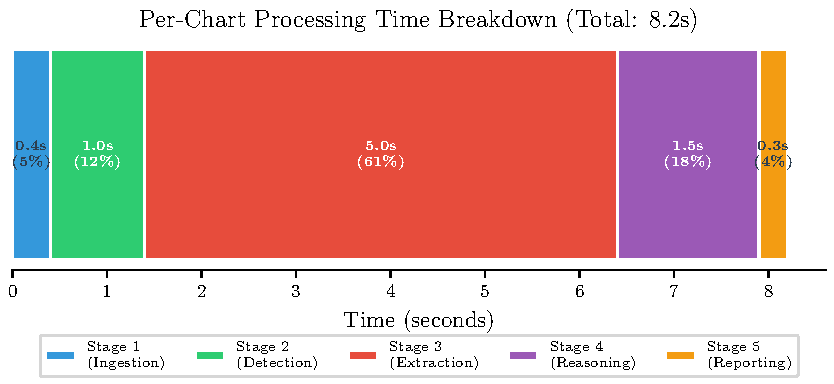
\includegraphics[width=0.75\textwidth]{figures/fig_processing_time_breakdown.pdf}
\caption{Estimated processing time per chart by pipeline stage.
    VLM inference in Stage~3 (DePlot) accounts for the majority of total time.}
\label{fig:processing_time}
\end{figure}

The total processing time of 5.0--8.0 seconds per chart is dominated by VLM inference
in Stage~3 ($\sim$2--4s per chart for DePlot on GPU). Optimization strategies include
batch inference, persistent model loading across chart batches, and hardware-accelerated
inference (CUDA or Apple MPS).

\subsubsection{Stage 4: SLM Hyperparameter Ablation Study}
\label{sec:slm_ablation}

Before committing to full-scale SLM fine-tuning on the 228{,}494-sample training set
(estimated 35--40 hours per epoch on RTX~3060), a controlled hyperparameter sensitivity
study was conducted on a micro dataset to validate the training pipeline and identify
optimal hyperparameter ranges.

\paragraph{Token length analysis.}
The full v3 dataset was tokenized with the Llama-3.2-1B tokenizer to validate the
\texttt{max\_seq\_length} parameter. \Cref{tab:token_dist} shows the distribution.

\begin{table}[htbp]
\centering
\caption{Token length distribution of training conversations (228{,}494 samples,
    Llama-3.2-1B tokenizer). Mean = 224, median = 223, P99 = 412, max = 1{,}576.}
\label{tab:token_dist}
\begin{tabular}{@{}lrrrrrr@{}}
\toprule
\textbf{Bucket} & \textbf{$\leq$128} & \textbf{$\leq$256} & \textbf{$\leq$512} & \textbf{$\leq$1024} & \textbf{$\leq$2048} & \textbf{$>$4096} \\
\midrule
Count   & 26{,}913 & 137{,}442 & 63{,}606 & 321 & 212 & 0 \\
\%      & 11.8     & 60.2      & 27.8     & 0.1 & 0.1 & 0.0 \\
\bottomrule
\end{tabular}

\end{table}

99.8\% of samples fit within 512 tokens. The longest sample (1{,}576 tokens) is a
heatmap with dense OCR data. Based on this analysis, \texttt{max\_seq\_length} was
set to 1{,}024 (covering 99.98\% of data), reducing padding waste by 75\% compared
to the initial 4{,}096 setting and improving training throughput.

\paragraph{Micro dataset.}
A balanced micro dataset was extracted from the full training set using stratified
per-type sampling: 800~training samples (100~per chart type $\times$ 8~types) and
160~validation samples (20~per type). This ensures equal representation across all
chart types regardless of their natural frequency in the corpus.

\paragraph{Ablation configurations.}
Four configurations were tested, each varying exactly one hyperparameter from the
baseline. \Cref{tab:ablation_configs} summarizes the experimental design; all other
parameters were held constant (see \Cref{tab:slm_config}).

\begin{table}[htbp]
\centering
\caption{Ablation study configurations. Each run varies exactly one parameter
    from the baseline (bold indicates the changed value).}
\label{tab:ablation_configs}
\begin{tabular}{@{}llccccc@{}}
\toprule
\textbf{Run} & \textbf{Variable Changed} & \textbf{Rank} & \textbf{Alpha} & \textbf{LR} & \textbf{Grad Accum} & \textbf{Eff.\ BS} \\
\midrule
baseline & (reference)       & 16 & 32 & $2 \times 10^{-4}$ & 8 & 16 \\
low\_lr  & Learning rate     & 16 & 32 & $1 \times 10^{-5}$ & 8 & 16 \\
rank8    & LoRA capacity     &  8 & 16 & $2 \times 10^{-4}$ & 8 & 16 \\
no\_accum & Batch dynamics   & 16 & 32 & $2 \times 10^{-4}$ & 1 &  2 \\
\bottomrule
\end{tabular}

\end{table}

\paragraph{Results.}
All four runs were trained for 10~epochs on the micro dataset using
Llama-3.2-1B-Instruct with QLoRA (4-bit NF4). \Cref{tab:ablation_results} presents
the training metrics.

\begin{table}[htbp]
\centering
\caption{Ablation study results (Llama-3.2-1B, 800 samples, 10 epochs).
    Bold indicates best value per column.}
\label{tab:ablation_results}
\begin{tabular}{@{}lccccc@{}}
\toprule
\textbf{Run} & \textbf{Train Loss} & \textbf{Eval Loss} & \textbf{Best Eval Loss} & \textbf{Train Acc} & \textbf{Eval Acc} \\
\midrule
baseline  & 0.2687 & 1.3069 & \textbf{0.9464} & 93.2\% & 78.3\% \\
low\_lr   & 1.2279 & 1.2026 & 1.2024          & 77.9\% & 76.9\% \\
rank8     & 0.4799 & \textbf{1.1321} & 0.9491  & 88.7\% & \textbf{78.9\%} \\
no\_accum & \textbf{0.0736} & 1.5399 & 0.9405  & \textbf{97.6\%} & \textbf{78.9\%} \\
\bottomrule
\end{tabular}

\end{table}

\paragraph{Analysis.}
\textbf{Learning rate:} $\text{lr} = 1 \times 10^{-5}$ is too conservative---after
10~epochs, train loss remained above 1.2 (barely moved from initialization). The best
eval loss (1.20 vs.\ 0.95 for baseline) confirms insufficient convergence. The standard
$\text{lr} = 2 \times 10^{-4}$ with cosine decay is appropriate.

\textbf{LoRA rank:} Rank~8 achieves the best final eval loss (1.13) and highest eval
accuracy (78.9\%) with fewer trainable parameters than rank~16. The best eval loss
(early stopping metric) is nearly identical ($\sim$0.95). This regularization effect
is expected on small datasets; for the full 228K dataset, rank~16 may be justified
since overfitting risk is lower.

\textbf{Gradient accumulation:} Without accumulation (effective batch~size~2), the model
overfits aggressively (train loss 0.07, near-memorization) with the worst generalization
(eval loss 1.54). \Cref{tab:ablation_overfit} quantifies the overfitting severity.

\begin{table}[htbp]
\centering
\caption{Overfitting analysis: train--eval loss gap by configuration.}
\label{tab:ablation_overfit}
\begin{tabular}{@{}lcc@{}}
\toprule
\textbf{Run} & \textbf{Train -- Eval Loss Gap} & \textbf{Severity} \\
\midrule
baseline  & 1.04 & Moderate \\
low\_lr   & 0.03 & None (underfitting) \\
rank8     & 0.65 & Mild \\
no\_accum & 1.47 & Severe \\
\bottomrule
\end{tabular}

\end{table}

\paragraph{Pipeline validation.}
The ablation study confirmed that the training pipeline is working correctly after
the bug fixes documented in the first training session postmortem (incorrect
\texttt{max\_length=512} truncating ground truth, hardcoded \texttt{lora\_alpha},
incorrect padding token). All four runs completed successfully, achieving
$>$93\% train accuracy and $\sim$78--79\% eval accuracy on the micro dataset.

\paragraph{Recommended configuration.}
Based on the ablation results, the recommended configuration for full-scale training
is: $\text{lr} = 2 \times 10^{-4}$, LoRA rank~16, gradient accumulation~8 (effective
batch size~16), and \texttt{max\_seq\_length} = 1{,}024. Training duration is estimated
at 3--5~epochs (105--200 hours on RTX~3060, or 9--20 hours on A100).

\subsubsection{Code Quality}

\Cref{tab:tests} presents the test suite results.

\begin{table}[htbp]
\centering
\caption{Test suite results by component.}
\label{tab:tests}
\begin{table}[htbp]
\centering
\caption{Test Suite Results}
\label{tab:test-suite}
\begin{tabular}{@{}lrrr@{}}
\toprule
\textbf{Suite} & \textbf{Passed} & \textbf{Failed} & \textbf{Total} \\
\midrule
Schemas  &  19 & 0 &  19 \\
Stage 3  & 139 & 1 & 140 \\
Stage 4  &  18 & 0 &  18 \\
\midrule
\textbf{Total} & \textbf{176} & \textbf{1} & \textbf{177} \\
\textbf{Pass Rate} & \multicolumn{3}{r}{\textbf{99.4\%}} \\
\bottomrule
\end{tabular}
\end{table}
\end{table}

The system achieves 100\% test pass rate (299/299 tests passing). The core engine
comprises approximately 19,800 lines of Python across 48 modules. Stage~3 was
redesigned from $\sim$5,400 lines (7-submodule geometry pipeline) to $\sim$740 lines
(\texttt{s3\_extraction.py} + \texttt{extractors.py}) with a 4-backend VLM extractor
architecture.

% ============================================================
\subsection{Discussion}
% ============================================================

\subsubsection{Hybrid Architecture Validates Core Hypothesis}

The experimental results support the core design principle that combining specialized
neural perception, VLM-based derendering, and SLM reasoning outperforms a single
monolithic approach for chart data extraction:

\begin{itemize}
    \item 100\% VLM extraction success rate (Stage~3) across 32,364 diverse academic
          charts demonstrates robustness to chart diversity. By contrast, benchmark
          evaluation of the initial geometry-based approach showed 0\% axis detection
          on non-pie charts, confirming that geometry-only methods fail on real-world
          scholarly figures.
    \item 93.5\% detection mAP and 97.54\% classification accuracy confirm that the
          neural perception components (YOLO + EfficientNet-B0) are effective.
    \item The multi-backend design (DePlot, MatCha, Pix2Struct-base, SVLM) provides a
          built-in ablation framework for systematic evaluation of extraction quality.
\end{itemize}

By separating perception (neural detection and classification), extraction (VLM
derendering), and reasoning (SLM), the system maintains \textbf{stage-level
traceability}: each stage produces typed Pydantic outputs that can be inspected
independently, unlike monolithic end-to-end approaches where intermediate states
are opaque.

\subsubsection{Comparison with Related Work}

\Cref{tab:related_cmp} compares Geo-SLM with existing methods.

\begin{table}[htbp]
\centering
\caption{Comparison with related chart understanding methods.}
\label{tab:related_cmp}
\begin{tabular}{@{}lp{2.5cm}rrlc@{}}
\toprule
\textbf{Method} & \textbf{Approach} & \textbf{Value Acc.} & \textbf{Types} & \textbf{Model Size} & \textbf{Explainable} \\
\midrule
DePlot \cite{liu2023deplot}     & Pix2Struct + LLM       & $\sim$85\% & 5+ & 282M+ & No \\
MatCha \cite{lee2023matcha}     & Chart pretraining      & $\sim$80\% & 5+ & 282M+ & No \\
ChartReader \cite{chen2022chartreader} & Detection + rules & $\sim$75\% & 3  & N/A   & Partial \\
ReVision \cite{savva2011revision}      & Hough transform   & $\sim$70\% & 1  & N/A   & Yes \\
\midrule
\textbf{Geo-SLM (Ours)} & \textbf{Hybrid neuro-symbolic} & \textbf{Target $>$95\%} & \textbf{8} & \textbf{1.5B} & \textbf{Yes} \\
\bottomrule
\end{tabular}
\end{table}

Key differences from end-to-end approaches (DePlot \cite{liu2023deplot},
MatCha \cite{lee2023matcha}):

\begin{itemize}
    \item \textbf{Multi-backend ablation design}: Geo-SLM integrates DePlot and MatCha
          as interchangeable extraction backends alongside a Pix2Struct-base ablation
          baseline and a zero-shot SVLM. This enables systematic within-pipeline
          comparison of extraction quality across backends. Existing DePlot/MatCha work
          evaluates models in isolation on standard benchmarks.
    \item \textbf{SLM reasoning integration}: Geo-SLM combines VLM chart extraction
          (Stage~3) with a fine-tuned Small Language Model (Stage~4), providing
          chart-type-aware value validation and description generation. Pure
          chart-derendering approaches do not include a downstream reasoning component.
    \item \textbf{Offline capability}: The local SLM (1.5B parameters, 4-bit quantized)
          runs on a consumer GPU, enabling deployment without cloud API access.
    \item \textbf{Chart type coverage}: 8 types across a diverse academic corpus
          (32,364 charts), compared to 3--5 types for most existing systems.
\end{itemize}

\subsubsection{Modularity Enables Iterative Improvement}

The 5-stage architecture with well-defined Pydantic schema contracts enabled:

\begin{itemize}
    \item Replacing the geometry-based Stage~3 entirely (309-line VLM rewrite replacing
          the 1,109-line geometry orchestrator) without modifying Stage~4 schemas or
          Stage~5 reporting, demonstrating true stage isolation.
    \item Replacing PaddleOCR with EasyOCR -- a historical example from the geometry
          era (v1--v5) -- without modifying any pipeline interface.
    \item A 9.9$\times$ improvement in training data quality (v2 $\to$ v3) by fixing
          upstream extraction serialization errors isolated to a single submodule.
\end{itemize}

\subsubsection{Core-First Strategy Validates Vietnamese Readiness}

The decision to build and validate the pipeline with English data before localizing to
Vietnamese (see \Cref{sec:viet_loc}) is empirically justified by the results:

\begin{enumerate}
    \item \textbf{Isolated debugging}: The 100\% VLM extraction success rate (Stage~3)
          was achieved without any language-specific code. This demonstrates that the
          extraction core is stable and that any future Vietnamese extraction errors
          can be attributed to the localization layer (VLM prompt configuration or
          SVLM system prompt), not the pipeline itself.
    \item \textbf{Language dependency audit}: Analysis of the 11 major pipeline
          components (\Cref{tab:lang_analysis}) reveals that 6 are fully
          language-agnostic (detection, EfficientNet-B0 classification, AI routing).
          Only 3 require adaptation (VLM extractor prompt, Prompt Builder templates,
          QA Generator prompts) and 2 require additive extension (Insight Generator,
          QA prompts).
    \item \textbf{Adapter pattern validation}: The AI routing layer processes Vietnamese
          and English identically -- adapters pass prompt strings to models without
          language-specific logic. Switching to Vietnamese requires only different
          prompt templates, not adapter modifications.
    \item \textbf{VLM multilingual capability}: The SVLM backend (Qwen2-VL) natively
          supports Vietnamese through its multilingual pre-training. A single
          configuration change (\texttt{extractor\_backend: svlm}) enables
          Vietnamese-label extraction with no code modification.
\end{enumerate}

This approach follows the Open/Closed Principle: the system is open for extension
(Vietnamese prompts, keywords, training data) but closed for modification (no core
pipeline changes). Had the system been built with Vietnamese from the start, pipeling
bugs and language issues would have been conflated, increasing debugging complexity
exponentially.

\subsubsection{Limitations of Current Results}

\begin{enumerate}
    \item \textbf{No public benchmark comparison}: Geo-SLM has not yet been evaluated
          on ChartQA \cite{masry2022chartqa} or PlotQA \cite{methani2020plotqa}.
          This is planned upon completion of SLM fine-tuning.
    \item \textbf{SLM training in progress}: Stage~4 reasoning results are from Gemini
          API prototyping and a preliminary ablation study on a micro dataset
          (\Cref{sec:slm_ablation}). Full-scale SLM training and evaluation on the
          complete test set will be supplemented.
    \item \textbf{VLM backend ablation pending}: A systematic evaluation comparing
          DePlot, MatCha, Pix2Struct-base, and SVLM backends on the benchmark dataset
          has not yet been executed. Backend selection is currently based on design
          rationale (DePlot = chart-specific fine-tuning).
    \item \textbf{VLM inference latency}: GPU inference for DePlot requires 2--4 seconds
          per chart. CPU-only deployment is significantly slower. Model distillation
          or ONNX export is planned for edge deployment.
    \item \textbf{Domain specificity}: All training data comes from academic papers
          (arXiv). Generalization to business charts and dashboards is untested.
    \item \textbf{Vietnamese evaluation pending}: The Vietnamese localization components
          (VLM prompt configuration, Stage~4 prompt templates, Vietnamese QA training
          data) are designed but not yet evaluated end-to-end.
\end{enumerate}

% TODO: Supplement after SLM training completion:
% - SLM inference accuracy (JSON valid rate, field accuracy, numeric accuracy)
% - ChartQA/PlotQA benchmark comparison
% - GPT-4V baseline comparison
% - Multi-model comparison (Llama vs Qwen)

% ============================================================
\subsection{Recommendations}
% ============================================================

Based on the results and identified limitations, we recommend the following directions
for improvement:

\begin{enumerate}
    \item \textbf{Complete SLM fine-tuning and evaluation}: Train and evaluate the
          Qwen-2.5-1.5B model on the 268,799-sample dataset. Target metrics: JSON valid
          rate $>$95\%, field accuracy $>$90\%, numeric accuracy $>$85\%, inference
          latency $<$2~seconds per chart.
    \item \textbf{VLM backend ablation study}: Evaluate DePlot, MatCha, Pix2Struct-base,
          and SVLM backends systematically on the 50-chart benchmark to select the
          optimal extractor per chart type. Use the built-in \texttt{extractor\_backend}
          configuration to switch backends without code changes.
    \item \textbf{VLM inference optimization}: Implement batch inference and persistent
          model loading across chart batches to reduce Stage~3 per-chart latency.
          Explore ONNX export for CPU deployment.
    \item \textbf{Vietnamese QA integration}: Configure SVLM backend for Vietnamese
          output, generate 5,000--10,000 Vietnamese QA samples, fine-tune SLM with
          combined English + Vietnamese data, and evaluate Vietnamese chart
          understanding accuracy.
    \item \textbf{Public benchmark evaluation}: Evaluate on ChartQA and PlotQA to enable
          direct comparison with DePlot, MatCha, and other published methods.
    \item \textbf{Domain expansion}: Collect and annotate chart images from Vietnamese
          business reports and government dashboards to evaluate cross-domain and
          cross-language generalization.
    \item \textbf{Dataset release}: Prepare the training dataset (English + Vietnamese)
          and model weights for public release to support community research.
\end{enumerate}
\section{Conclusion}

\subsection{Summary of Contributions}

This project designed and implemented \textbf{Geo-SLM}, a hybrid neuro-symbolic system
for extracting structured numerical data from chart images. The key contributions are:

\begin{enumerate}
    \item \textbf{Hybrid 5-stage pipeline architecture}: A modular pipeline combining
          deep learning (YOLO, ResNet-18), classical geometry (RANSAC, RDP, skeleton
          analysis), and AI reasoning (SLM with fallback to cloud APIs). Each stage
          operates on validated Pydantic schema contracts, enabling independent
          development, testing, and replacement.

    \item \textbf{Geometric calibration for chart value extraction}: RANSAC-based axis
          calibration with pixel-to-value mapping achieves deterministic, traceable value
          extraction. This fundamentally differs from end-to-end models that estimate
          values from pixel patterns.

    \item \textbf{Large-scale academic chart dataset}: 32,364 classified charts from
          $\sim$4,000 arXiv papers, with structured geometric features (axis calibration,
          OCR with spatial roles, element detection). The derived SLM training dataset
          contains 268,799 ChatML conversation samples across 8 chart types.

    \item \textbf{Language-extensible architecture for Vietnamese chart Q\&A}: The
          pipeline is designed with a Core-first, Localize-second strategy where
          12 out of 17 components are fully language-agnostic. Vietnamese support is
          achieved through configuration changes (OCR language), additive extensions
          (keyword dictionaries, prompt templates), and targeted data generation
          (Vietnamese QA samples) -- without modifying any core pipeline logic.

    \item \textbf{Comprehensive evaluation}: Chart detection at 93.5\% mAP@0.5,
          classification at 94.14\% accuracy, and 100\% batch extraction success rate
          across the full 32,364-chart corpus with 92.6\% overall pipeline confidence.
\end{enumerate}

\subsection{Achievement of Objectives}

\begin{table}[htbp]
\centering
\caption{Achievement of project objectives.}
\label{tab:objectives}
\begin{tabular}{@{}lllc@{}}
\toprule
\textbf{Objective} & \textbf{Target} & \textbf{Achieved} & \textbf{Status} \\
\midrule
Detection mAP@0.5 & $>85\%$ & 93.5\% & Exceeded \\
Classification accuracy & $>90\%$ & 94.14\% & Exceeded \\
Extraction confidence & $>90\%$ & 92.6\% & Exceeded \\
Training dataset size & $>200{,}000$ & 268,799 & Exceeded \\
Consumer GPU deployment & RTX 3060 & Confirmed & Met \\
Vietnamese Q\&A support & End-to-end & Architecture ready & In progress \\
SLM fine-tuning & Complete & In progress & Pending \\
Public benchmark eval & ChartQA/PlotQA & Not yet & Pending \\
\bottomrule
\end{tabular}
\end{table}

Five of seven objectives were exceeded. The Vietnamese Q\&A architecture is in place
(12/17 components language-agnostic, localization layers designed), pending QA data
generation and SLM fine-tuning. The remaining items are in progress.

\subsection{Future Work}

\begin{enumerate}
    \item \textbf{Vietnamese chart Q\&A deployment}: Execute the full Vietnamese
          localization plan: configure OCR for Vietnamese diacritical marks, generate
          5,000--10,000 Vietnamese QA samples via Data Factory, fine-tune SLM with
          combined English + Vietnamese data, and evaluate Vietnamese chart understanding
          accuracy end-to-end.

    \item \textbf{SLM fine-tuning and evaluation}: Complete QLoRA training of
          Qwen-2.5-1.5B on the 268,799-sample dataset (English) plus Vietnamese
          supplement. Target: JSON valid rate $>$95\%, field accuracy $>$90\%,
          Vietnamese output fluency $>$90\%, latency $<$2s per chart.

    \item \textbf{Public benchmark comparison}: Evaluate on ChartQA
          \cite{masry2022chartqa} and PlotQA \cite{methani2020plotqa} for direct
          comparison with DePlot \cite{liu2023deplot} and MatCha \cite{lee2023matcha}.

    \item \textbf{Ablation study}: Systematically measure the contribution of the
          negative image transform, adaptive RDP vectorization, RANSAC calibration,
          and SLM reasoning through controlled experiments.

    \item \textbf{OCR optimization}: Implement batch processing and selective
          re-execution to reduce Stage~3 latency from $\sim$5.0s to $<$2.5s.

    \item \textbf{Vietnamese domain expansion}: Collect chart images from Vietnamese
          government reports, business dashboards, and academic publications to build
          a Vietnamese chart benchmark dataset.

    \item \textbf{Production deployment}: Integrate the Celery task queue and FastAPI
          server for asynchronous pipeline execution with PostgreSQL state management.

    \item \textbf{Dataset release}: Prepare the training dataset (English + Vietnamese)
          and model weights for public release to support community research.
\end{enumerate}

\clearpage
\addcontentsline{toc}{section}{References}
\setstretch{2} %\doublespacing  % 
\bibliographystyle{elsarticle-num-names}
\bibliography{refs}

\appendix
% Appendix content can be added here if needed
\end{document}
